% Update slides, version 5 (26 Nov 2026):
%   direct (LU) vs iterative solvers on the kinetic system with ONE radial
%   cell, all 9 snapshots, L1 (Pitagora job 2919298) and L2 (job 2919325)
%   (run_compare_solvers_nr1_cluster.sh, iface/TestKineticSolversSerial.cpp);
%   raw output in v5_2919298/compare_solvers_nr1_L1.txt and
%   v5_2919325/compare_solvers_nr1_L2.txt.
%   Parallel, one radius split over 1-64 ranks, L2 (job 2919644,
%   run_scaling_nr1_cluster.sh, iface/TestKineticHypreRadius.cpp): data in
%   v5_2919644/scaling_nr1_L2.csv, figure and table from
%   v5_2919644/plot_scaling_nr1.py.
%   L4 (27 Nov 2026): serial comparison, job 2919957, in
%   v5_2919957_L4/compare_solvers_nr1_L4.txt; parallel scaling (the job after
%   it) in v5_2919957_L4/scaling_nr1_L4.csv, figure from
%   plot_scaling_nr1.py ... --ref compare_solvers_nr1_L4.txt.
% Include with % Update slides, version 5 (26 Nov 2026):
%   direct (LU) vs iterative solvers on the kinetic system with ONE radial
%   cell, all 9 snapshots, L1 (Pitagora job 2919298) and L2 (job 2919325)
%   (run_compare_solvers_nr1_cluster.sh, iface/TestKineticSolversSerial.cpp);
%   raw output in v5_2919298/compare_solvers_nr1_L1.txt and
%   v5_2919325/compare_solvers_nr1_L2.txt.
%   Parallel, one radius split over 1-64 ranks, L2 (job 2919644,
%   run_scaling_nr1_cluster.sh, iface/TestKineticHypreRadius.cpp): data in
%   v5_2919644/scaling_nr1_L2.csv, figure and table from
%   v5_2919644/plot_scaling_nr1.py.
%   L4 (27 Nov 2026): serial comparison, job 2919957, in
%   v5_2919957_L4/compare_solvers_nr1_L4.txt; parallel scaling (the job after
%   it) in v5_2919957_L4/scaling_nr1_L4.csv, figure from
%   plot_scaling_nr1.py ... --ref compare_solvers_nr1_L4.txt.
% Include with % Update slides, version 5 (26 Nov 2026):
%   direct (LU) vs iterative solvers on the kinetic system with ONE radial
%   cell, all 9 snapshots, L1 (Pitagora job 2919298) and L2 (job 2919325)
%   (run_compare_solvers_nr1_cluster.sh, iface/TestKineticSolversSerial.cpp);
%   raw output in v5_2919298/compare_solvers_nr1_L1.txt and
%   v5_2919325/compare_solvers_nr1_L2.txt.
%   Parallel, one radius split over 1-64 ranks, L2 (job 2919644,
%   run_scaling_nr1_cluster.sh, iface/TestKineticHypreRadius.cpp): data in
%   v5_2919644/scaling_nr1_L2.csv, figure and table from
%   v5_2919644/plot_scaling_nr1.py.
%   L4 (27 Nov 2026): serial comparison, job 2919957, in
%   v5_2919957_L4/compare_solvers_nr1_L4.txt; parallel scaling (the job after
%   it) in v5_2919957_L4/scaling_nr1_L4.csv, figure from
%   plot_scaling_nr1.py ... --ref compare_solvers_nr1_L4.txt.
% Include with % Update slides, version 5 (26 Nov 2026):
%   direct (LU) vs iterative solvers on the kinetic system with ONE radial
%   cell, all 9 snapshots, L1 (Pitagora job 2919298) and L2 (job 2919325)
%   (run_compare_solvers_nr1_cluster.sh, iface/TestKineticSolversSerial.cpp);
%   raw output in v5_2919298/compare_solvers_nr1_L1.txt and
%   v5_2919325/compare_solvers_nr1_L2.txt.
%   Parallel, one radius split over 1-64 ranks, L2 (job 2919644,
%   run_scaling_nr1_cluster.sh, iface/TestKineticHypreRadius.cpp): data in
%   v5_2919644/scaling_nr1_L2.csv, figure and table from
%   v5_2919644/plot_scaling_nr1.py.
%   L4 (27 Nov 2026): serial comparison, job 2919957, in
%   v5_2919957_L4/compare_solvers_nr1_L4.txt; parallel scaling (the job after
%   it) in v5_2919957_L4/scaling_nr1_L4.csv, figure from
%   plot_scaling_nr1.py ... --ref compare_solvers_nr1_L4.txt.
% Include with \input{update_frames_v5} (update_2026-11-26.tex).

% ---------------------------------------------------------------------
\begin{frame}{Direct vs iterative, one radius: setup}
    \footnotesize
    \begin{itemize}
        \item kinetic system only ($f_\mathrm{hot}$, $f_\mathrm{re}$), \textbf{one radial cell} ($N_r = 1$),
              analytic toroidal geometry, three resolutions
        \begin{itemize}
            \item L1: $N = 38\,000$ unknowns ($f_\mathrm{hot}$ $250 \times 32 = 8\,000$,
                  $f_\mathrm{re}$ $150 \times 200 = 30\,000$), $1.8\times10^{5}$ nonzeros
            \item L2: $N = 152\,000$ ($f_\mathrm{hot}$ $32\,000$ + $f_\mathrm{re}$ $120\,000$),
                  $7.2\times10^{5}$ nonzeros
            \item L4: $N = 2.43$\,M ($f_\mathrm{hot}$ $0.51$\,M + $f_\mathrm{re}$ $1.92$\,M),
                  $1.16\times10^{7}$ nonzeros
            \item no radial coupling: what is left is the momentum-space $(p, \xi)$ operator
        \end{itemize}
        \item all 9 snapshots: injection start / end, CQ at 5, 10, 20, 29, 40, 49\,ms and end
        \begin{itemize}
            \item $\Delta t = 1.8\times10^{-7}$\,s (injection), $1.0\times10^{-7}$\,s (CQ, DREAM substep)
            \item first time step, matrix dumped by \texttt{dreami} (\texttt{-dream\_save\_system})
        \end{itemize}
        \item serial (Pitagora, one core), zero initial guess, restart 100,
              stop at $\|r\|/\|b\| < 10^{-10}$ (true residual)
        \item solvers
        \begin{enumerate}
            \item \textbf{LU}: direct factorization (PETSc's own LU; MUMPS not available in this PETSc build)
            \item \textbf{AMG + GMRES}: one BoomerAMG V-cycle per iteration
            \item \textbf{ILU(0) + GMRES}
            \item \textbf{[GMRES + AMG/Euclid ILU(1)] + FGMRES}: the MIRadialBJ block solver, here with a single block
        \end{enumerate}
    \end{itemize}
\end{frame}

% ---------------------------------------------------------------------
\begin{frame}{Direct vs iterative, one radius: results (serial, L1)}
    \small
    \begin{center}
    \resizebox{\linewidth}{!}{%
    \begin{tabular}{l|r|rr|rr|rr}
        \hline
        & LU & \multicolumn{2}{c|}{AMG + GMRES} & \multicolumn{2}{c|}{ILU(0) + GMRES}
        & \multicolumn{2}{c}{[GMRES+AMG/Eu(1)] + FGMRES} \\
        snapshot & time [ms] & its & time [ms] & its & time [ms] & its (inner) & time [ms] \\
        \hline
        injection start & 123 & 7 & 32 &  9 & \textbf{15} & 2 (6) & 72 \\
        injection end   & 132 & 9 & 39 & 12 & \textbf{18} & 2 (6) & 75 \\
        CQ 5\,ms        & 132 & 8 & 36 & 10 & \textbf{16} & 2 (6) & 76 \\
        CQ 10\,ms       & 174 & 8 & 36 & 10 & \textbf{15} & 2 (6) & 74 \\
        CQ 20\,ms       & 132 & 8 & 36 & 10 & \textbf{15} & 2 (6) & 75 \\
        CQ 29\,ms       & 131 & 7 & 33 &  9 & \textbf{14} & 2 (6) & 76 \\
        CQ 40\,ms       & 131 & 7 & 33 &  9 & \textbf{14} & 2 (6) & 74 \\
        CQ 49\,ms       & 130 & 7 & 33 &  9 & \textbf{14} & 1 (3) & 65 \\
        CQ end          & 129 & 8 & 36 &  8 & \textbf{13} & 2 (4) & 70 \\
        \hline
        relative error  & $\leq 2\times10^{-12}$ & \multicolumn{2}{c|}{$\leq 2\times10^{-10}$}
                        & \multicolumn{2}{c|}{$\leq 2\times10^{-11}$} & \multicolumn{2}{c}{$\leq 4\times10^{-11}$} \\
        \hline
    \end{tabular}}
    \end{center}
    \vspace{0.3em}
    \begin{itemize}
        \item time = setup + solve; error = $\|x - x_\mathrm{ref}\| / \|x_\mathrm{ref}\|$,
              $x_\mathrm{ref}$ = \texttt{dreami}'s solution
        \item every solver converges on every snapshot
        \item LU: factorization 122--173\,ms, triangular solves 1\,ms
        \item block-Jacobi variants with one block give the same iterations and residuals
              as the global ones (consistency check)
    \end{itemize}
\end{frame}

% ---------------------------------------------------------------------
\begin{frame}{Direct vs iterative, one radius: results (serial, L2)}
    \small
    \begin{center}
    \resizebox{\linewidth}{!}{%
    \begin{tabular}{l|r|rr|rr|rr}
        \hline
        & LU & \multicolumn{2}{c|}{AMG + GMRES} & \multicolumn{2}{c|}{ILU(0) + GMRES}
        & \multicolumn{2}{c}{[GMRES+AMG/Eu(1)] + FGMRES} \\
        snapshot & time [ms] & its & time [ms] & its & time [ms] & its (inner) & time [ms] \\
        \hline
        injection start & 638 & 10 & 167 & 15 & \textbf{92}  & 2 (18) & 380 \\
        injection end   & 720 & 11 & 186 & 19 & \textbf{116} & 2 (6)  & 281 \\
        CQ 5\,ms        & 709 & 11 & 182 & 15 & \textbf{91}  & 2 (6)  & 281 \\
        CQ 10\,ms       & 709 & 11 & 181 & 15 & \textbf{90}  & 2 (6)  & 280 \\
        CQ 20\,ms       & 703 & 11 & 183 & 14 & \textbf{86}  & 2 (6)  & 281 \\
        CQ 29\,ms       & 706 & 11 & 183 & 14 & \textbf{86}  & 2 (6)  & 274 \\
        CQ 40\,ms       & 701 & 11 & 186 & 14 & \textbf{85}  & 2 (6)  & 287 \\
        CQ 49\,ms       & 690 & \textbf{58} & \textbf{928} & 13 & \textbf{82} & 2 (6) & 274 \\
        CQ end          & 667 & 10 & 166 & 11 & \textbf{69}  & 2 (6)  & 258 \\
        \hline
        relative error  & $\leq 3\times10^{-12}$ & \multicolumn{2}{c|}{$\leq 5\times10^{-9}$}
                        & \multicolumn{2}{c|}{$\leq 5\times10^{-10}$} & \multicolumn{2}{c}{$\leq 3\times10^{-12}$} \\
        \hline
    \end{tabular}}
    \end{center}
    \vspace{0.3em}
    \begin{itemize}
        \item every solver converges on every snapshot
        \item LU: factorization 0.63--0.71\,s, triangular solves 6\,ms
        \item AMG + GMRES at CQ 49\,ms: 58 iterations, and its true residual $9\times10^{-10}$
              stays above the $10^{-10}$ target (error $5\times10^{-9}$)
    \end{itemize}
\end{frame}

% ---------------------------------------------------------------------
\begin{frame}{Direct vs iterative, one radius: results (serial, L4)}
    \small
    \begin{center}
    \resizebox{\linewidth}{!}{%
    \begin{tabular}{l|r|rr|rr|rr}
        \hline
        & LU & \multicolumn{2}{c|}{AMG + GMRES} & \multicolumn{2}{c|}{ILU(0) + GMRES}
        & \multicolumn{2}{c}{[GMRES+AMG/Eu(1)] + FGMRES} \\
        snapshot & time [s] & its & time [s] & its & time [s] & its (inner) & time [s] \\
        \hline
        injection start & 17.5 & \textbf{104} & \textbf{31.2} & 56 & \textbf{6.4} & 2 (\textbf{260}) & \textbf{60.1} \\
        injection end   & 22.0 & 14  & \textbf{4.5}  & 61 & 7.2  & 2 (7) & 5.4 \\
        CQ 5\,ms        & 21.1 & 13  & \textbf{4.0}  & 40 & 4.4  & 2 (6) & 5.0 \\
        CQ 10\,ms       & 21.0 & 22  & 6.4  & 40 & \textbf{4.2}  & 2 (6) & 5.0 \\
        CQ 20\,ms       & 20.9 & 13  & \textbf{4.0}  & 39 & 4.2  & 2 (6) & 5.0 \\
        CQ 29\,ms       & 21.0 & \textbf{107} & \textbf{33.6} & 38 & \textbf{4.1} & 2 (6) & 4.9 \\
        CQ 40\,ms       & 20.8 & 13  & 4.0  & 37 & \textbf{3.9}  & 2 (6) & 4.8 \\
        CQ 49\,ms       & 20.3 & 13  & 4.0  & 31 & \textbf{3.3}  & 2 (6) & 4.8 \\
        CQ end          & 18.3 & 13  & 3.8  & 26 & \textbf{2.6}  & 2 (6) & 4.5 \\
        \hline
        relative error  & $\leq 7\times10^{-11}$ & \multicolumn{2}{c|}{$\leq 5\times10^{-10}$}
                        & \multicolumn{2}{c|}{$\leq 6\times10^{-10}$} & \multicolumn{2}{c}{$\leq 6\times10^{-11}$} \\
        \hline
    \end{tabular}}
    \end{center}
    \vspace{0.3em}
    \begin{itemize}
        \item every solver converges on every snapshot (injection end: no reference solution, no error)
        \item LU: factorization 17--22\,s, triangular solves 0.13\,s
        \item AMG + GMRES and the MIRadialBJ block solver have outliers ($8\times$ / $12\times$ slower);
              ILU(0) + GMRES has none, but its iterations grow with the resolution (26--61)
        \item true residual $\approx 10^{-8}$ for every solver, LU included: the floor of these systems at L4
    \end{itemize}
\end{frame}

% ---------------------------------------------------------------------
\begin{frame}{Direct vs iterative, one radius: conclusions}
    \footnotesize
    \begin{center}
    \begin{tabular}{l|rr|r}
        \hline
        total time, range over the 9 snapshots & L1 [ms] & L2 [ms] & L4 [s] \\
        \hline
        LU                                  & 123--174 & 638--720 & 17.5--22.0 \\
        AMG + GMRES                         & 32--39   & 166--186 (928) & 3.8--6.4 (31, 34) \\
        ILU(0) + GMRES                      & \textbf{13--18} & \textbf{69--116} & \textbf{2.6--7.2} \\
        {[GMRES+AMG/Eu(1)] + FGMRES}        & 65--76   & 258--380 & 4.5--5.4 (60) \\
        \hline
        unknowns                            & 38\,k & 152\,k & 2.43\,M \\
        \hline
    \end{tabular}
    \end{center}
    \vspace{0.2em}
    \begin{itemize}
        \item \textbf{ILU(0) + GMRES is the fastest and the only one without outliers}: $8$--$9\times$ faster
              than LU at L1--L2, $\approx 5\times$ at L4; at L4 AMG + GMRES is as fast on most snapshots;
              ILU iterations grow with the resolution: 8--12 (L1), 11--19 (L2), 26--61 (L4)
        \item \textbf{LU is the slowest}: almost all the time is the factorization; it would pay off
              only if reused for $\gtrsim 10$ solves, but the matrix changes at every time step
        \item \textbf{AMG + GMRES is not robust}: 7--22 iterations, except 58 (L2, CQ 49\,ms)
              and 104--107 (L4, injection start, CQ 29\,ms)
        \item the MIRadialBJ block solver: 2 outer iterations on every snapshot and level, but its
              AMG + Euclid setup dominates (50\,ms L1, 200\,ms L2, 3.4\,s L4); L4 injection start: 260 inner its
    \end{itemize}
    \vspace{0.2em}
    \textbf{Caveat}: easy systems ($\Delta t \approx 10^{-7}$\,s, no radial coupling); with $N_r = 11$ at L2 (v4)
    ILU(0) needed 150--238 iterations. Next: full source step ($\Delta t \approx 10^{-4}$\,s), LU with MUMPS
\end{frame}

% =====================================================================
% Parallel: one radius split over the MPI ranks
% =====================================================================
\begin{frame}{Parallel, one radius: speed-up (L2)}
    \footnotesize
    $N_r = 1$, L2 ($152\,000$ unknowns): the single radius block is split over all $n$ ranks
    (1 exclusive node, $n = 1 \dots 64$), solved by a parallel BoomerAMG; 9 snapshots, 2 repeats
    \begin{center}
        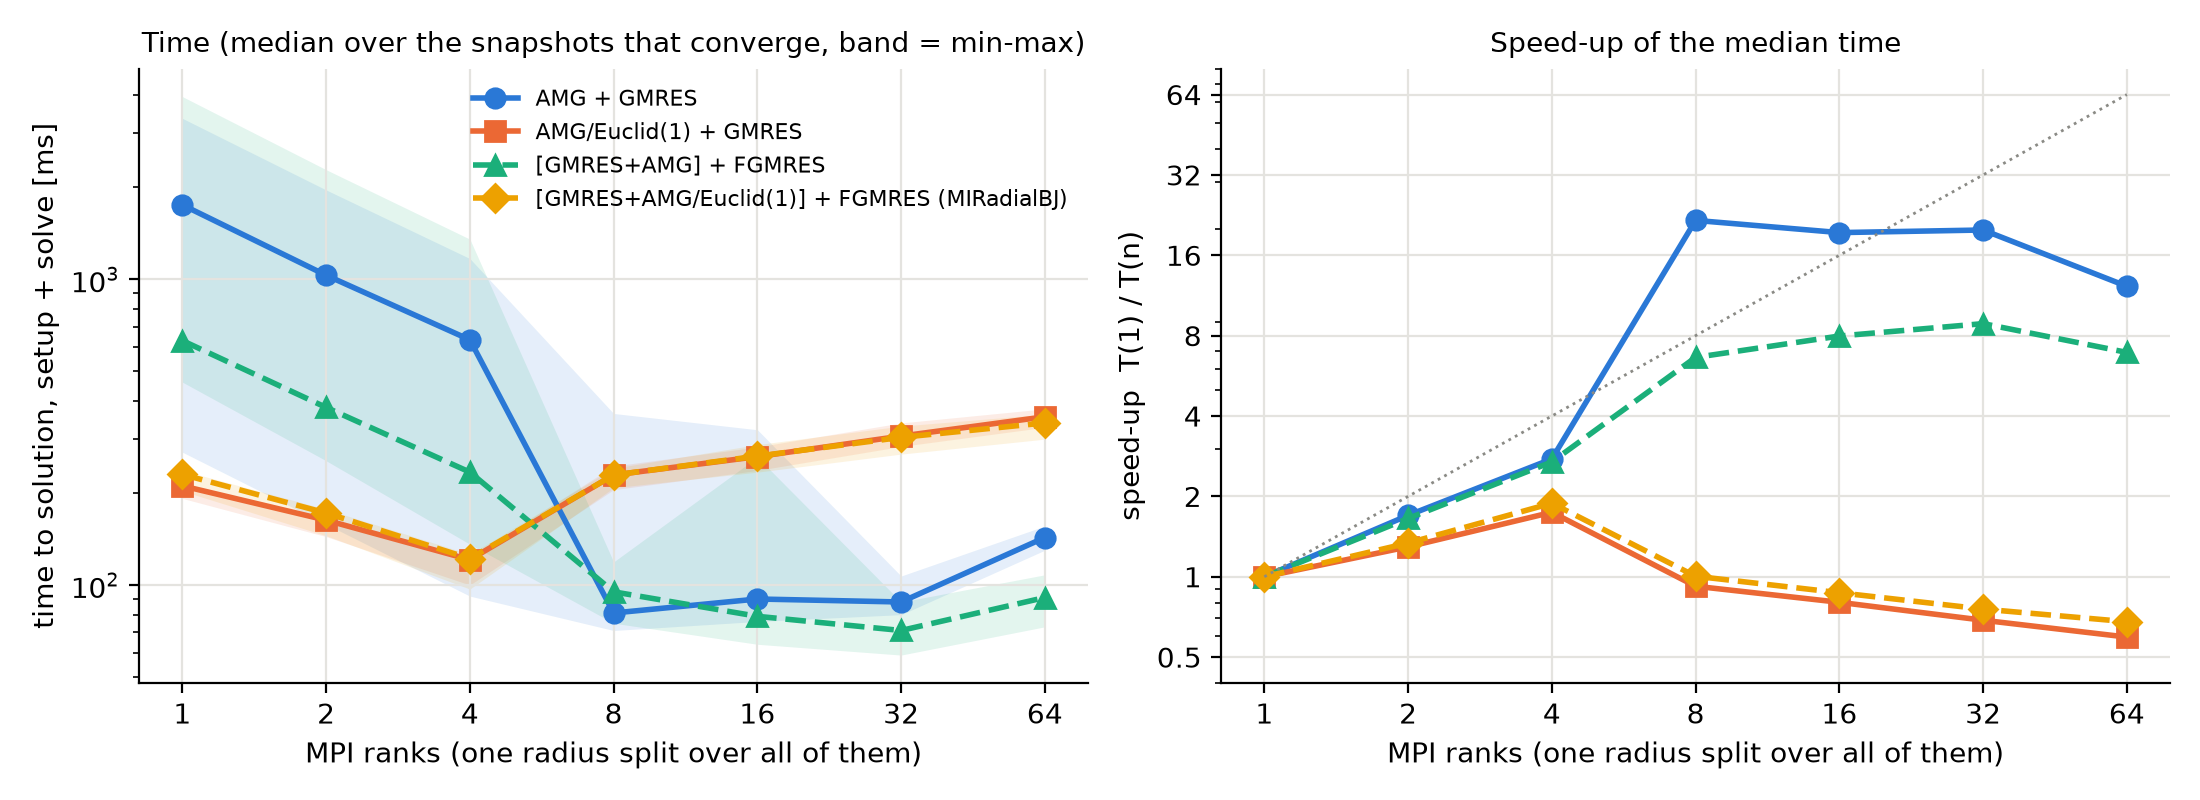
\includegraphics[width=0.95\linewidth]{v5_2919644/scaling_nr1_L2}
    \end{center}
    \vspace{-0.6em}
    \begin{itemize}
        \item time = setup + solve, best of 2 repeats; median over the snapshots that converge;
              speed-up of the median time
        \item AMG + GMRES (default smoother): the jump at 8 ranks is \textbf{not parallel efficiency}:
              its iterations drop from up to 237 (and 2 divergences) on 1--4 ranks to 15--21
    \end{itemize}
\end{frame}

% ---------------------------------------------------------------------
\begin{frame}{Parallel, one radius: results (L2)}
    \footnotesize
    \begin{center}
    \resizebox{\linewidth}{!}{%
    \begin{tabular}{l|rrrrrrr}
        \hline
        median time [ms] (iterations) & 1 & 2 & 4 & 8 & 16 & 32 & 64 \\
        \hline
        AMG + GMRES                 & 1751$^*$ & 1031$^*$ & 634$^*$ & 81 & 90 & 88 & 143 \\
                                    & (20--237) & & & (15--111) & (17--114) & (12--21) & (13--21) \\
        AMG/Euclid(1) + GMRES       & 211 & 163 & \textbf{121} & 229 & 263 & 307 & 355 \\
                                    & (3--4) & (3--4) & (3--4) & (7--9) & (9--12) & (8--14) & (10--12) \\
        {[GMRES+AMG] + FGMRES}      & 630$^*$ & 381$^*$ & 234$^*$ & 95 & 79 & \textbf{71} & 91 \\
        {[GMRES+AMG/Euclid(1)] + FGMRES} & 230 & 172 & \textbf{122} & 229 & 264 & 304 & 339 \\
        \hline
    \end{tabular}}
    \end{center}
    \vspace{-0.4em}
    {\scriptsize FGMRES variants: 2 outer iterations everywhere.
    $^*$ CQ 10\,ms and CQ 29\,ms diverge on 1--4 ranks with the default smoother (not in the median).}
    \begin{itemize}
        \item \textbf{Euclid smoother}: 3--4 iterations, fastest on 1--4 ranks, best speed-up $1.9\times$ at 4 ranks;
              beyond that its parallel ILU setup grows (90\,ms at 4 $\to$ 280\,ms at 64 ranks) and the
              iterations triple: \textbf{slower with more ranks}
        \item \textbf{default smoother}: unreliable on 1--4 ranks, then 71--95\,ms from 8 to 32 ranks,
              slower again at 64
        \item best parallel time $\approx 71$\,ms (32 ranks) vs \textbf{90\,ms for serial ILU(0) + GMRES} on one core
              (previous slides): splitting one radius buys at most $\approx 1.3\times$
        \item $152\,000$ unknowns over 64 ranks is $\approx 2\,400$ rows per rank: communication and
              setup dominate. Parallelism should come from the radius ($N_r \geq$ ranks), not from inside it
        \item to check: AMG + GMRES (default smoother) took 10--11 iterations on the same matrices in the
              serial test, which has no extra \texttt{-scale diag}
    \end{itemize}
\end{frame}

% ---------------------------------------------------------------------
\begin{frame}{Parallel, one radius: speed-up (L4)}
    \footnotesize
    $N_r = 1$, L4 ($2.43$\,M unknowns, 38\,000 rows per rank at 64 ranks), 1 exclusive node,
    8 snapshots (injection end: no reference solution), 2 repeats
    \begin{center}
        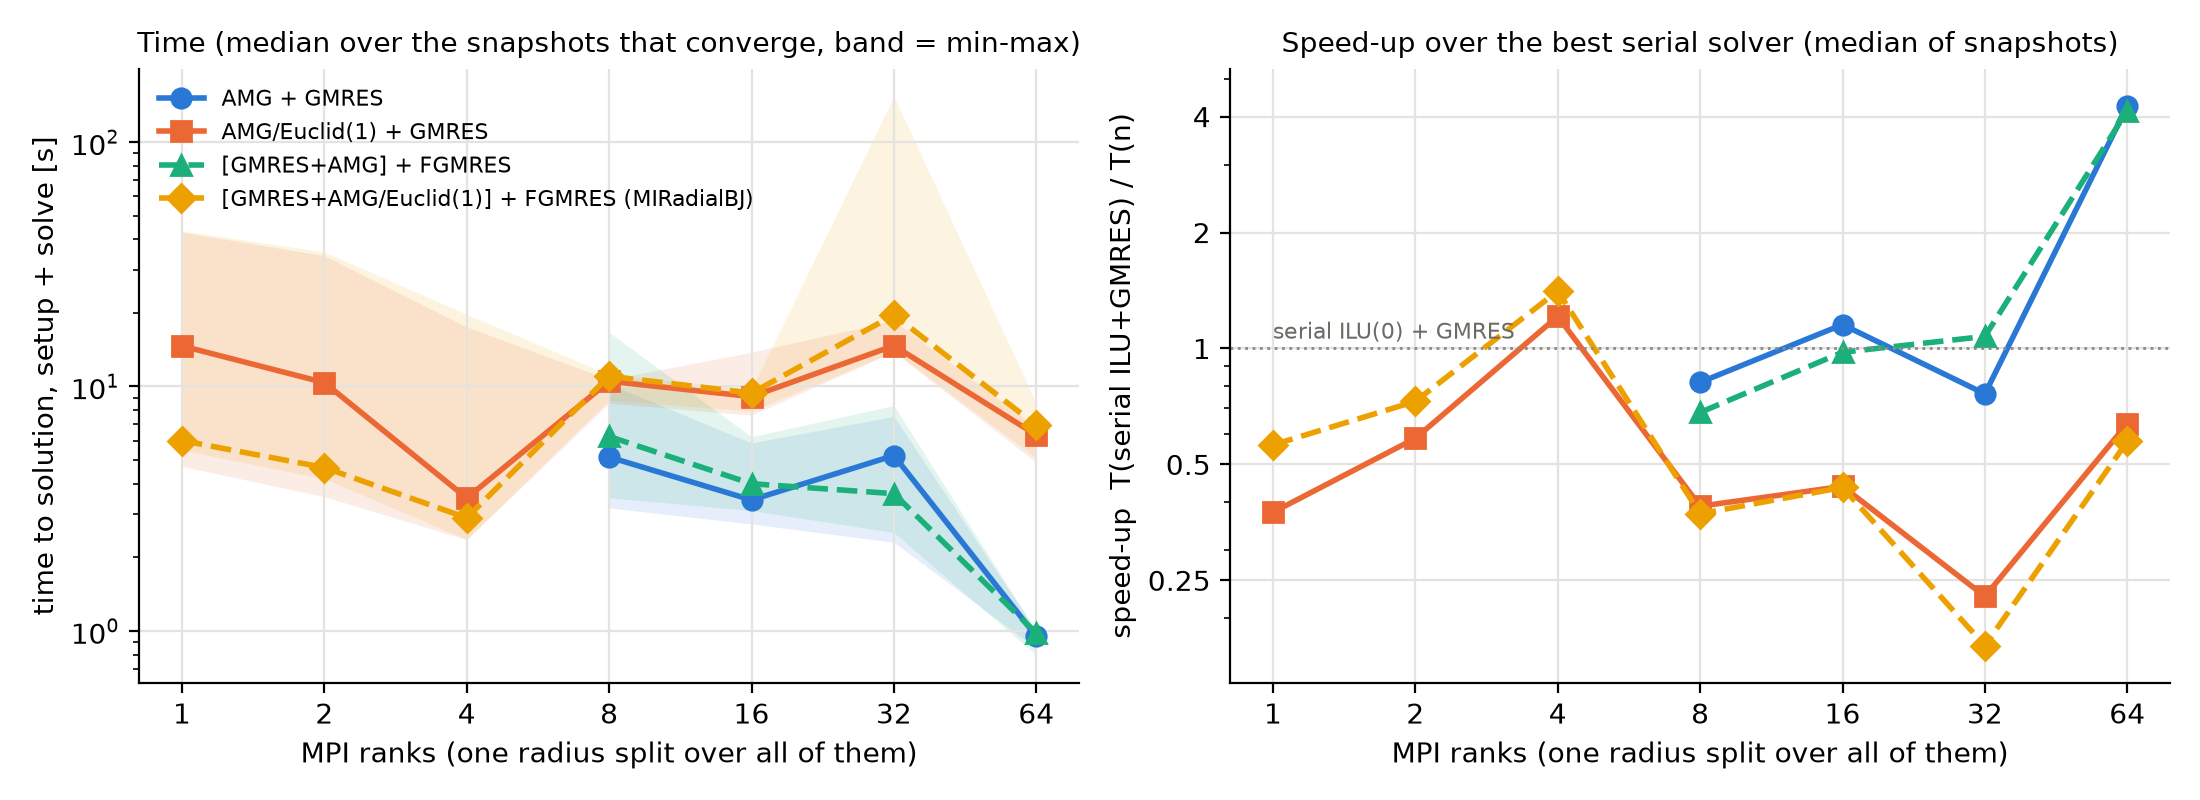
\includegraphics[width=0.95\linewidth]{v5_2919957_L4/scaling_nr1_L4}
    \end{center}
    \vspace{-0.6em}
    \begin{itemize}
        \item speed-up here = per snapshot, time of \textbf{serial ILU(0) + GMRES} (one core, 2.6--7.2\,s) / time on $n$ ranks:
              T(1) does not exist for the default smoother, which fails on 1--4 ranks
        \item a run counts if it converges \textbf{and} its true residual is $\leq 10^{-4}$; no point where more than half of the snapshots fail
    \end{itemize}
\end{frame}

% ---------------------------------------------------------------------
\begin{frame}{Parallel, one radius: results (L4)}
    \footnotesize
    \begin{center}
    \resizebox{\linewidth}{!}{%
    \begin{tabular}{l|rrrrrrr}
        \hline
        median time [s] (iterations) & 1 & 2 & 4 & 8 & 16 & 32 & 64 \\
        \hline
        AMG + GMRES                 & fail 7/8 & fail 7/8 & fail 7/8 & 5.1$^*$ & 3.4 & 5.2 & \textbf{0.95} \\
                                    & & & & (22--133) & (25--121) & (33--252) & (14--20) \\
        AMG/Euclid(1) + GMRES       & 14.7 & 10.4 & 3.5$^*$ & 10.5 & 9.1 & 14.7$^*$ & 6.3$^*$ \\
                                    & (10--206) & (10--206) & (11--206) & (9--15) & (12--109) & (188--292) & (35--61) \\
        {[GMRES+AMG] + FGMRES}      & fail 7/8 & fail 7/8 & fail 7/8 & 6.2$^*$ & 4.0 & 3.6 & \textbf{0.98} \\
        {[GMRES+AMG/Euclid(1)] + FGMRES} & 6.0 & 4.7 & 2.9$^*$ & 11.0 & 9.4 & 19.6$^*$ & 6.9 \\
        \hline
        serial ILU(0) + GMRES (one core) & \multicolumn{7}{l}{4.1 (median), 2.6--6.4} \\
        \hline
    \end{tabular}}
    \end{center}
    \vspace{-0.4em}
    {\scriptsize $^*$ 1--3 of the 8 snapshots fail (not in the median). FGMRES variants: 2 outer iterations.}
    \begin{itemize}
        \item \textbf{default smoother}: fails on 1--4 ranks, converges from 8 on; at \textbf{64 ranks all 8 snapshots
              in 0.8--1.0\,s}: $4\times$ faster than serial ILU(0) + GMRES, $20\times$ faster than serial LU
        \item not monotonic: at 32 ranks AMG + GMRES needs 143--252 iterations (the AMG hierarchy changes with the partition)
        \item \textbf{Euclid smoother}: best at 4 ranks (2.9\,s, $1.4\times$ serial ILU); from 8 ranks its setup jumps
              from 1\,s to 8--10\,s and at 32 ranks 2--3 snapshots fail: \textbf{does not scale}
        \item unlike L2, splitting one radius pays off at L4 (38\,000 rows per rank at 64 ranks), but only with the default smoother
    \end{itemize}
\end{frame}

% ---------------------------------------------------------------------
\begin{frame}{Parallel, one radius: open issues}
    \small
    \begin{itemize}
        \item \textbf{the default smoother fails on 1--4 ranks in the parallel test}
              (L2: 2 of 9 snapshots, L4: 7 of 8), \textbf{but not in the serial test} on the same matrices:
              there AMG + GMRES converges in 7--22 iterations on almost every snapshot
        \begin{itemize}
            \item with one radius both run GMRES + block Jacobi (1 block) + one BoomerAMG V-cycle, right
                  preconditioning; the difference is the extra \texttt{-scale diag} of the parallel test
                  (it solves $D^{-1}A$, which also changes the AMG hierarchy and the stopping test)
            \item until this is understood, the 1--4 rank points of the default smoother are not reliable
        \end{itemize}
        \item \textbf{``converged'' is not enough}: the parallel test stops on the residual of the scaled
              system; at L4, 64 ranks, AMG/Euclid + GMRES reports convergence with true residual $10^{-2}$
              (here counted as a failure; the AMG V-cycle variants often stop at $10^{-6}$--$10^{-5}$)
        \item next: repeat the 1--64 rank scan with \texttt{-scale none} at L2 and L4
    \end{itemize}
\end{frame}
 (update_2026-11-26.tex).

% ---------------------------------------------------------------------
\begin{frame}{Direct vs iterative, one radius: setup}
    \footnotesize
    \begin{itemize}
        \item kinetic system only ($f_\mathrm{hot}$, $f_\mathrm{re}$), \textbf{one radial cell} ($N_r = 1$),
              analytic toroidal geometry, three resolutions
        \begin{itemize}
            \item L1: $N = 38\,000$ unknowns ($f_\mathrm{hot}$ $250 \times 32 = 8\,000$,
                  $f_\mathrm{re}$ $150 \times 200 = 30\,000$), $1.8\times10^{5}$ nonzeros
            \item L2: $N = 152\,000$ ($f_\mathrm{hot}$ $32\,000$ + $f_\mathrm{re}$ $120\,000$),
                  $7.2\times10^{5}$ nonzeros
            \item L4: $N = 2.43$\,M ($f_\mathrm{hot}$ $0.51$\,M + $f_\mathrm{re}$ $1.92$\,M),
                  $1.16\times10^{7}$ nonzeros
            \item no radial coupling: what is left is the momentum-space $(p, \xi)$ operator
        \end{itemize}
        \item all 9 snapshots: injection start / end, CQ at 5, 10, 20, 29, 40, 49\,ms and end
        \begin{itemize}
            \item $\Delta t = 1.8\times10^{-7}$\,s (injection), $1.0\times10^{-7}$\,s (CQ, DREAM substep)
            \item first time step, matrix dumped by \texttt{dreami} (\texttt{-dream\_save\_system})
        \end{itemize}
        \item serial (Pitagora, one core), zero initial guess, restart 100,
              stop at $\|r\|/\|b\| < 10^{-10}$ (true residual)
        \item solvers
        \begin{enumerate}
            \item \textbf{LU}: direct factorization (PETSc's own LU; MUMPS not available in this PETSc build)
            \item \textbf{AMG + GMRES}: one BoomerAMG V-cycle per iteration
            \item \textbf{ILU(0) + GMRES}
            \item \textbf{[GMRES + AMG/Euclid ILU(1)] + FGMRES}: the MIRadialBJ block solver, here with a single block
        \end{enumerate}
    \end{itemize}
\end{frame}

% ---------------------------------------------------------------------
\begin{frame}{Direct vs iterative, one radius: results (serial, L1)}
    \small
    \begin{center}
    \resizebox{\linewidth}{!}{%
    \begin{tabular}{l|r|rr|rr|rr}
        \hline
        & LU & \multicolumn{2}{c|}{AMG + GMRES} & \multicolumn{2}{c|}{ILU(0) + GMRES}
        & \multicolumn{2}{c}{[GMRES+AMG/Eu(1)] + FGMRES} \\
        snapshot & time [ms] & its & time [ms] & its & time [ms] & its (inner) & time [ms] \\
        \hline
        injection start & 123 & 7 & 32 &  9 & \textbf{15} & 2 (6) & 72 \\
        injection end   & 132 & 9 & 39 & 12 & \textbf{18} & 2 (6) & 75 \\
        CQ 5\,ms        & 132 & 8 & 36 & 10 & \textbf{16} & 2 (6) & 76 \\
        CQ 10\,ms       & 174 & 8 & 36 & 10 & \textbf{15} & 2 (6) & 74 \\
        CQ 20\,ms       & 132 & 8 & 36 & 10 & \textbf{15} & 2 (6) & 75 \\
        CQ 29\,ms       & 131 & 7 & 33 &  9 & \textbf{14} & 2 (6) & 76 \\
        CQ 40\,ms       & 131 & 7 & 33 &  9 & \textbf{14} & 2 (6) & 74 \\
        CQ 49\,ms       & 130 & 7 & 33 &  9 & \textbf{14} & 1 (3) & 65 \\
        CQ end          & 129 & 8 & 36 &  8 & \textbf{13} & 2 (4) & 70 \\
        \hline
        relative error  & $\leq 2\times10^{-12}$ & \multicolumn{2}{c|}{$\leq 2\times10^{-10}$}
                        & \multicolumn{2}{c|}{$\leq 2\times10^{-11}$} & \multicolumn{2}{c}{$\leq 4\times10^{-11}$} \\
        \hline
    \end{tabular}}
    \end{center}
    \vspace{0.3em}
    \begin{itemize}
        \item time = setup + solve; error = $\|x - x_\mathrm{ref}\| / \|x_\mathrm{ref}\|$,
              $x_\mathrm{ref}$ = \texttt{dreami}'s solution
        \item every solver converges on every snapshot
        \item LU: factorization 122--173\,ms, triangular solves 1\,ms
        \item block-Jacobi variants with one block give the same iterations and residuals
              as the global ones (consistency check)
    \end{itemize}
\end{frame}

% ---------------------------------------------------------------------
\begin{frame}{Direct vs iterative, one radius: results (serial, L2)}
    \small
    \begin{center}
    \resizebox{\linewidth}{!}{%
    \begin{tabular}{l|r|rr|rr|rr}
        \hline
        & LU & \multicolumn{2}{c|}{AMG + GMRES} & \multicolumn{2}{c|}{ILU(0) + GMRES}
        & \multicolumn{2}{c}{[GMRES+AMG/Eu(1)] + FGMRES} \\
        snapshot & time [ms] & its & time [ms] & its & time [ms] & its (inner) & time [ms] \\
        \hline
        injection start & 638 & 10 & 167 & 15 & \textbf{92}  & 2 (18) & 380 \\
        injection end   & 720 & 11 & 186 & 19 & \textbf{116} & 2 (6)  & 281 \\
        CQ 5\,ms        & 709 & 11 & 182 & 15 & \textbf{91}  & 2 (6)  & 281 \\
        CQ 10\,ms       & 709 & 11 & 181 & 15 & \textbf{90}  & 2 (6)  & 280 \\
        CQ 20\,ms       & 703 & 11 & 183 & 14 & \textbf{86}  & 2 (6)  & 281 \\
        CQ 29\,ms       & 706 & 11 & 183 & 14 & \textbf{86}  & 2 (6)  & 274 \\
        CQ 40\,ms       & 701 & 11 & 186 & 14 & \textbf{85}  & 2 (6)  & 287 \\
        CQ 49\,ms       & 690 & \textbf{58} & \textbf{928} & 13 & \textbf{82} & 2 (6) & 274 \\
        CQ end          & 667 & 10 & 166 & 11 & \textbf{69}  & 2 (6)  & 258 \\
        \hline
        relative error  & $\leq 3\times10^{-12}$ & \multicolumn{2}{c|}{$\leq 5\times10^{-9}$}
                        & \multicolumn{2}{c|}{$\leq 5\times10^{-10}$} & \multicolumn{2}{c}{$\leq 3\times10^{-12}$} \\
        \hline
    \end{tabular}}
    \end{center}
    \vspace{0.3em}
    \begin{itemize}
        \item every solver converges on every snapshot
        \item LU: factorization 0.63--0.71\,s, triangular solves 6\,ms
        \item AMG + GMRES at CQ 49\,ms: 58 iterations, and its true residual $9\times10^{-10}$
              stays above the $10^{-10}$ target (error $5\times10^{-9}$)
    \end{itemize}
\end{frame}

% ---------------------------------------------------------------------
\begin{frame}{Direct vs iterative, one radius: results (serial, L4)}
    \small
    \begin{center}
    \resizebox{\linewidth}{!}{%
    \begin{tabular}{l|r|rr|rr|rr}
        \hline
        & LU & \multicolumn{2}{c|}{AMG + GMRES} & \multicolumn{2}{c|}{ILU(0) + GMRES}
        & \multicolumn{2}{c}{[GMRES+AMG/Eu(1)] + FGMRES} \\
        snapshot & time [s] & its & time [s] & its & time [s] & its (inner) & time [s] \\
        \hline
        injection start & 17.5 & \textbf{104} & \textbf{31.2} & 56 & \textbf{6.4} & 2 (\textbf{260}) & \textbf{60.1} \\
        injection end   & 22.0 & 14  & \textbf{4.5}  & 61 & 7.2  & 2 (7) & 5.4 \\
        CQ 5\,ms        & 21.1 & 13  & \textbf{4.0}  & 40 & 4.4  & 2 (6) & 5.0 \\
        CQ 10\,ms       & 21.0 & 22  & 6.4  & 40 & \textbf{4.2}  & 2 (6) & 5.0 \\
        CQ 20\,ms       & 20.9 & 13  & \textbf{4.0}  & 39 & 4.2  & 2 (6) & 5.0 \\
        CQ 29\,ms       & 21.0 & \textbf{107} & \textbf{33.6} & 38 & \textbf{4.1} & 2 (6) & 4.9 \\
        CQ 40\,ms       & 20.8 & 13  & 4.0  & 37 & \textbf{3.9}  & 2 (6) & 4.8 \\
        CQ 49\,ms       & 20.3 & 13  & 4.0  & 31 & \textbf{3.3}  & 2 (6) & 4.8 \\
        CQ end          & 18.3 & 13  & 3.8  & 26 & \textbf{2.6}  & 2 (6) & 4.5 \\
        \hline
        relative error  & $\leq 7\times10^{-11}$ & \multicolumn{2}{c|}{$\leq 5\times10^{-10}$}
                        & \multicolumn{2}{c|}{$\leq 6\times10^{-10}$} & \multicolumn{2}{c}{$\leq 6\times10^{-11}$} \\
        \hline
    \end{tabular}}
    \end{center}
    \vspace{0.3em}
    \begin{itemize}
        \item every solver converges on every snapshot (injection end: no reference solution, no error)
        \item LU: factorization 17--22\,s, triangular solves 0.13\,s
        \item AMG + GMRES and the MIRadialBJ block solver have outliers ($8\times$ / $12\times$ slower);
              ILU(0) + GMRES has none, but its iterations grow with the resolution (26--61)
        \item true residual $\approx 10^{-8}$ for every solver, LU included: the floor of these systems at L4
    \end{itemize}
\end{frame}

% ---------------------------------------------------------------------
\begin{frame}{Direct vs iterative, one radius: conclusions}
    \footnotesize
    \begin{center}
    \begin{tabular}{l|rr|r}
        \hline
        total time, range over the 9 snapshots & L1 [ms] & L2 [ms] & L4 [s] \\
        \hline
        LU                                  & 123--174 & 638--720 & 17.5--22.0 \\
        AMG + GMRES                         & 32--39   & 166--186 (928) & 3.8--6.4 (31, 34) \\
        ILU(0) + GMRES                      & \textbf{13--18} & \textbf{69--116} & \textbf{2.6--7.2} \\
        {[GMRES+AMG/Eu(1)] + FGMRES}        & 65--76   & 258--380 & 4.5--5.4 (60) \\
        \hline
        unknowns                            & 38\,k & 152\,k & 2.43\,M \\
        \hline
    \end{tabular}
    \end{center}
    \vspace{0.2em}
    \begin{itemize}
        \item \textbf{ILU(0) + GMRES is the fastest and the only one without outliers}: $8$--$9\times$ faster
              than LU at L1--L2, $\approx 5\times$ at L4; at L4 AMG + GMRES is as fast on most snapshots;
              ILU iterations grow with the resolution: 8--12 (L1), 11--19 (L2), 26--61 (L4)
        \item \textbf{LU is the slowest}: almost all the time is the factorization; it would pay off
              only if reused for $\gtrsim 10$ solves, but the matrix changes at every time step
        \item \textbf{AMG + GMRES is not robust}: 7--22 iterations, except 58 (L2, CQ 49\,ms)
              and 104--107 (L4, injection start, CQ 29\,ms)
        \item the MIRadialBJ block solver: 2 outer iterations on every snapshot and level, but its
              AMG + Euclid setup dominates (50\,ms L1, 200\,ms L2, 3.4\,s L4); L4 injection start: 260 inner its
    \end{itemize}
    \vspace{0.2em}
    \textbf{Caveat}: easy systems ($\Delta t \approx 10^{-7}$\,s, no radial coupling); with $N_r = 11$ at L2 (v4)
    ILU(0) needed 150--238 iterations. Next: full source step ($\Delta t \approx 10^{-4}$\,s), LU with MUMPS
\end{frame}

% =====================================================================
% Parallel: one radius split over the MPI ranks
% =====================================================================
\begin{frame}{Parallel, one radius: speed-up (L2)}
    \footnotesize
    $N_r = 1$, L2 ($152\,000$ unknowns): the single radius block is split over all $n$ ranks
    (1 exclusive node, $n = 1 \dots 64$), solved by a parallel BoomerAMG; 9 snapshots, 2 repeats
    \begin{center}
        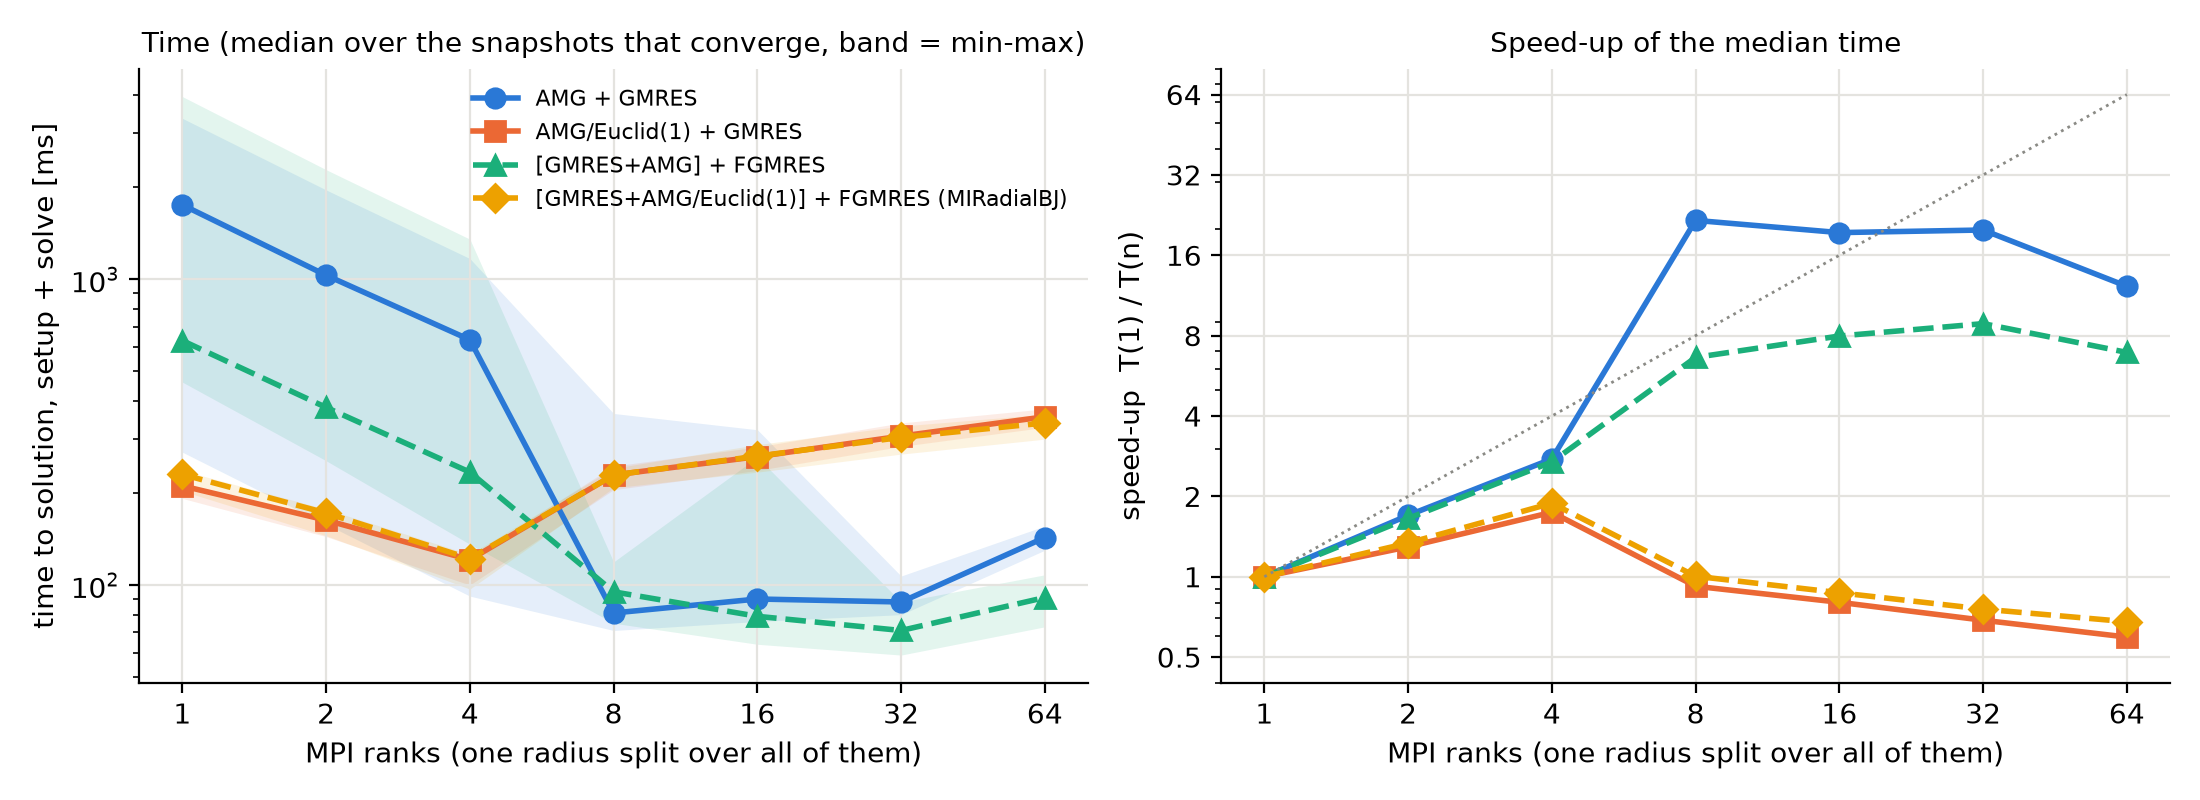
\includegraphics[width=0.95\linewidth]{v5_2919644/scaling_nr1_L2}
    \end{center}
    \vspace{-0.6em}
    \begin{itemize}
        \item time = setup + solve, best of 2 repeats; median over the snapshots that converge;
              speed-up of the median time
        \item AMG + GMRES (default smoother): the jump at 8 ranks is \textbf{not parallel efficiency}:
              its iterations drop from up to 237 (and 2 divergences) on 1--4 ranks to 15--21
    \end{itemize}
\end{frame}

% ---------------------------------------------------------------------
\begin{frame}{Parallel, one radius: results (L2)}
    \footnotesize
    \begin{center}
    \resizebox{\linewidth}{!}{%
    \begin{tabular}{l|rrrrrrr}
        \hline
        median time [ms] (iterations) & 1 & 2 & 4 & 8 & 16 & 32 & 64 \\
        \hline
        AMG + GMRES                 & 1751$^*$ & 1031$^*$ & 634$^*$ & 81 & 90 & 88 & 143 \\
                                    & (20--237) & & & (15--111) & (17--114) & (12--21) & (13--21) \\
        AMG/Euclid(1) + GMRES       & 211 & 163 & \textbf{121} & 229 & 263 & 307 & 355 \\
                                    & (3--4) & (3--4) & (3--4) & (7--9) & (9--12) & (8--14) & (10--12) \\
        {[GMRES+AMG] + FGMRES}      & 630$^*$ & 381$^*$ & 234$^*$ & 95 & 79 & \textbf{71} & 91 \\
        {[GMRES+AMG/Euclid(1)] + FGMRES} & 230 & 172 & \textbf{122} & 229 & 264 & 304 & 339 \\
        \hline
    \end{tabular}}
    \end{center}
    \vspace{-0.4em}
    {\scriptsize FGMRES variants: 2 outer iterations everywhere.
    $^*$ CQ 10\,ms and CQ 29\,ms diverge on 1--4 ranks with the default smoother (not in the median).}
    \begin{itemize}
        \item \textbf{Euclid smoother}: 3--4 iterations, fastest on 1--4 ranks, best speed-up $1.9\times$ at 4 ranks;
              beyond that its parallel ILU setup grows (90\,ms at 4 $\to$ 280\,ms at 64 ranks) and the
              iterations triple: \textbf{slower with more ranks}
        \item \textbf{default smoother}: unreliable on 1--4 ranks, then 71--95\,ms from 8 to 32 ranks,
              slower again at 64
        \item best parallel time $\approx 71$\,ms (32 ranks) vs \textbf{90\,ms for serial ILU(0) + GMRES} on one core
              (previous slides): splitting one radius buys at most $\approx 1.3\times$
        \item $152\,000$ unknowns over 64 ranks is $\approx 2\,400$ rows per rank: communication and
              setup dominate. Parallelism should come from the radius ($N_r \geq$ ranks), not from inside it
        \item to check: AMG + GMRES (default smoother) took 10--11 iterations on the same matrices in the
              serial test, which has no extra \texttt{-scale diag}
    \end{itemize}
\end{frame}

% ---------------------------------------------------------------------
\begin{frame}{Parallel, one radius: speed-up (L4)}
    \footnotesize
    $N_r = 1$, L4 ($2.43$\,M unknowns, 38\,000 rows per rank at 64 ranks), 1 exclusive node,
    8 snapshots (injection end: no reference solution), 2 repeats
    \begin{center}
        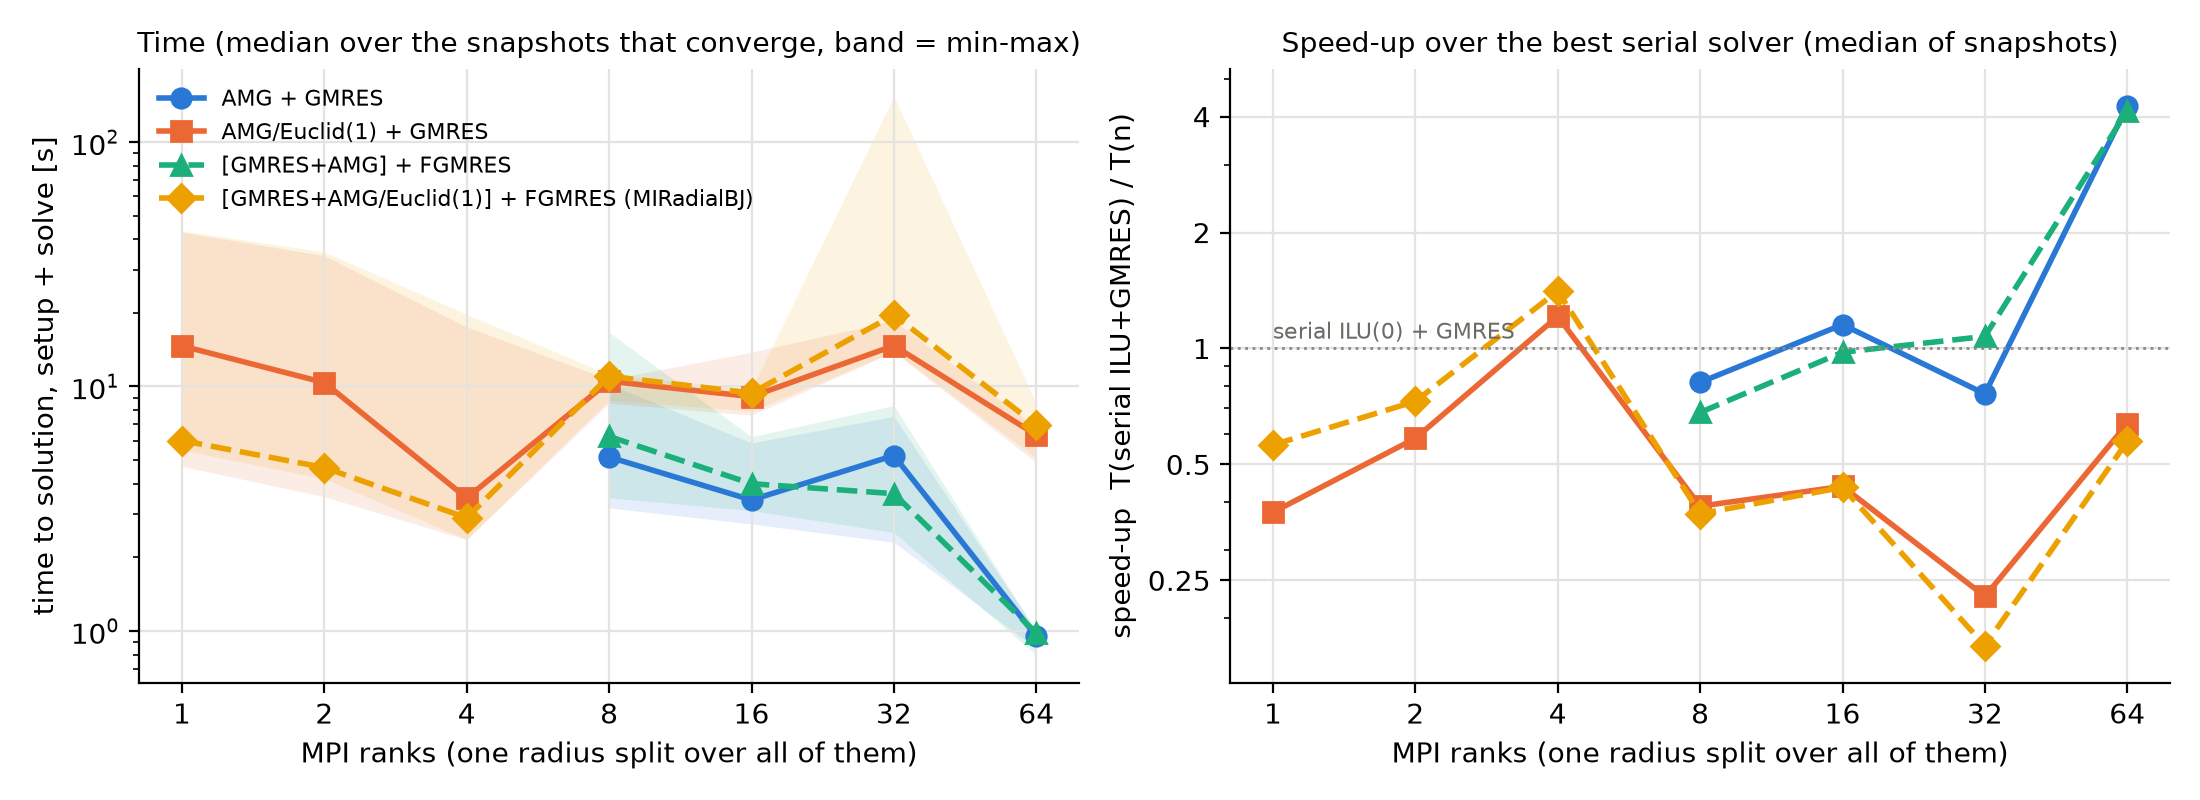
\includegraphics[width=0.95\linewidth]{v5_2919957_L4/scaling_nr1_L4}
    \end{center}
    \vspace{-0.6em}
    \begin{itemize}
        \item speed-up here = per snapshot, time of \textbf{serial ILU(0) + GMRES} (one core, 2.6--7.2\,s) / time on $n$ ranks:
              T(1) does not exist for the default smoother, which fails on 1--4 ranks
        \item a run counts if it converges \textbf{and} its true residual is $\leq 10^{-4}$; no point where more than half of the snapshots fail
    \end{itemize}
\end{frame}

% ---------------------------------------------------------------------
\begin{frame}{Parallel, one radius: results (L4)}
    \footnotesize
    \begin{center}
    \resizebox{\linewidth}{!}{%
    \begin{tabular}{l|rrrrrrr}
        \hline
        median time [s] (iterations) & 1 & 2 & 4 & 8 & 16 & 32 & 64 \\
        \hline
        AMG + GMRES                 & fail 7/8 & fail 7/8 & fail 7/8 & 5.1$^*$ & 3.4 & 5.2 & \textbf{0.95} \\
                                    & & & & (22--133) & (25--121) & (33--252) & (14--20) \\
        AMG/Euclid(1) + GMRES       & 14.7 & 10.4 & 3.5$^*$ & 10.5 & 9.1 & 14.7$^*$ & 6.3$^*$ \\
                                    & (10--206) & (10--206) & (11--206) & (9--15) & (12--109) & (188--292) & (35--61) \\
        {[GMRES+AMG] + FGMRES}      & fail 7/8 & fail 7/8 & fail 7/8 & 6.2$^*$ & 4.0 & 3.6 & \textbf{0.98} \\
        {[GMRES+AMG/Euclid(1)] + FGMRES} & 6.0 & 4.7 & 2.9$^*$ & 11.0 & 9.4 & 19.6$^*$ & 6.9 \\
        \hline
        serial ILU(0) + GMRES (one core) & \multicolumn{7}{l}{4.1 (median), 2.6--6.4} \\
        \hline
    \end{tabular}}
    \end{center}
    \vspace{-0.4em}
    {\scriptsize $^*$ 1--3 of the 8 snapshots fail (not in the median). FGMRES variants: 2 outer iterations.}
    \begin{itemize}
        \item \textbf{default smoother}: fails on 1--4 ranks, converges from 8 on; at \textbf{64 ranks all 8 snapshots
              in 0.8--1.0\,s}: $4\times$ faster than serial ILU(0) + GMRES, $20\times$ faster than serial LU
        \item not monotonic: at 32 ranks AMG + GMRES needs 143--252 iterations (the AMG hierarchy changes with the partition)
        \item \textbf{Euclid smoother}: best at 4 ranks (2.9\,s, $1.4\times$ serial ILU); from 8 ranks its setup jumps
              from 1\,s to 8--10\,s and at 32 ranks 2--3 snapshots fail: \textbf{does not scale}
        \item unlike L2, splitting one radius pays off at L4 (38\,000 rows per rank at 64 ranks), but only with the default smoother
    \end{itemize}
\end{frame}

% ---------------------------------------------------------------------
\begin{frame}{Parallel, one radius: open issues}
    \small
    \begin{itemize}
        \item \textbf{the default smoother fails on 1--4 ranks in the parallel test}
              (L2: 2 of 9 snapshots, L4: 7 of 8), \textbf{but not in the serial test} on the same matrices:
              there AMG + GMRES converges in 7--22 iterations on almost every snapshot
        \begin{itemize}
            \item with one radius both run GMRES + block Jacobi (1 block) + one BoomerAMG V-cycle, right
                  preconditioning; the difference is the extra \texttt{-scale diag} of the parallel test
                  (it solves $D^{-1}A$, which also changes the AMG hierarchy and the stopping test)
            \item until this is understood, the 1--4 rank points of the default smoother are not reliable
        \end{itemize}
        \item \textbf{``converged'' is not enough}: the parallel test stops on the residual of the scaled
              system; at L4, 64 ranks, AMG/Euclid + GMRES reports convergence with true residual $10^{-2}$
              (here counted as a failure; the AMG V-cycle variants often stop at $10^{-6}$--$10^{-5}$)
        \item next: repeat the 1--64 rank scan with \texttt{-scale none} at L2 and L4
    \end{itemize}
\end{frame}
 (update_2026-11-26.tex).

% ---------------------------------------------------------------------
\begin{frame}{Direct vs iterative, one radius: setup}
    \footnotesize
    \begin{itemize}
        \item kinetic system only ($f_\mathrm{hot}$, $f_\mathrm{re}$), \textbf{one radial cell} ($N_r = 1$),
              analytic toroidal geometry, three resolutions
        \begin{itemize}
            \item L1: $N = 38\,000$ unknowns ($f_\mathrm{hot}$ $250 \times 32 = 8\,000$,
                  $f_\mathrm{re}$ $150 \times 200 = 30\,000$), $1.8\times10^{5}$ nonzeros
            \item L2: $N = 152\,000$ ($f_\mathrm{hot}$ $32\,000$ + $f_\mathrm{re}$ $120\,000$),
                  $7.2\times10^{5}$ nonzeros
            \item L4: $N = 2.43$\,M ($f_\mathrm{hot}$ $0.51$\,M + $f_\mathrm{re}$ $1.92$\,M),
                  $1.16\times10^{7}$ nonzeros
            \item no radial coupling: what is left is the momentum-space $(p, \xi)$ operator
        \end{itemize}
        \item all 9 snapshots: injection start / end, CQ at 5, 10, 20, 29, 40, 49\,ms and end
        \begin{itemize}
            \item $\Delta t = 1.8\times10^{-7}$\,s (injection), $1.0\times10^{-7}$\,s (CQ, DREAM substep)
            \item first time step, matrix dumped by \texttt{dreami} (\texttt{-dream\_save\_system})
        \end{itemize}
        \item serial (Pitagora, one core), zero initial guess, restart 100,
              stop at $\|r\|/\|b\| < 10^{-10}$ (true residual)
        \item solvers
        \begin{enumerate}
            \item \textbf{LU}: direct factorization (PETSc's own LU; MUMPS not available in this PETSc build)
            \item \textbf{AMG + GMRES}: one BoomerAMG V-cycle per iteration
            \item \textbf{ILU(0) + GMRES}
            \item \textbf{[GMRES + AMG/Euclid ILU(1)] + FGMRES}: the MIRadialBJ block solver, here with a single block
        \end{enumerate}
    \end{itemize}
\end{frame}

% ---------------------------------------------------------------------
\begin{frame}{Direct vs iterative, one radius: results (serial, L1)}
    \small
    \begin{center}
    \resizebox{\linewidth}{!}{%
    \begin{tabular}{l|r|rr|rr|rr}
        \hline
        & LU & \multicolumn{2}{c|}{AMG + GMRES} & \multicolumn{2}{c|}{ILU(0) + GMRES}
        & \multicolumn{2}{c}{[GMRES+AMG/Eu(1)] + FGMRES} \\
        snapshot & time [ms] & its & time [ms] & its & time [ms] & its (inner) & time [ms] \\
        \hline
        injection start & 123 & 7 & 32 &  9 & \textbf{15} & 2 (6) & 72 \\
        injection end   & 132 & 9 & 39 & 12 & \textbf{18} & 2 (6) & 75 \\
        CQ 5\,ms        & 132 & 8 & 36 & 10 & \textbf{16} & 2 (6) & 76 \\
        CQ 10\,ms       & 174 & 8 & 36 & 10 & \textbf{15} & 2 (6) & 74 \\
        CQ 20\,ms       & 132 & 8 & 36 & 10 & \textbf{15} & 2 (6) & 75 \\
        CQ 29\,ms       & 131 & 7 & 33 &  9 & \textbf{14} & 2 (6) & 76 \\
        CQ 40\,ms       & 131 & 7 & 33 &  9 & \textbf{14} & 2 (6) & 74 \\
        CQ 49\,ms       & 130 & 7 & 33 &  9 & \textbf{14} & 1 (3) & 65 \\
        CQ end          & 129 & 8 & 36 &  8 & \textbf{13} & 2 (4) & 70 \\
        \hline
        relative error  & $\leq 2\times10^{-12}$ & \multicolumn{2}{c|}{$\leq 2\times10^{-10}$}
                        & \multicolumn{2}{c|}{$\leq 2\times10^{-11}$} & \multicolumn{2}{c}{$\leq 4\times10^{-11}$} \\
        \hline
    \end{tabular}}
    \end{center}
    \vspace{0.3em}
    \begin{itemize}
        \item time = setup + solve; error = $\|x - x_\mathrm{ref}\| / \|x_\mathrm{ref}\|$,
              $x_\mathrm{ref}$ = \texttt{dreami}'s solution
        \item every solver converges on every snapshot
        \item LU: factorization 122--173\,ms, triangular solves 1\,ms
        \item block-Jacobi variants with one block give the same iterations and residuals
              as the global ones (consistency check)
    \end{itemize}
\end{frame}

% ---------------------------------------------------------------------
\begin{frame}{Direct vs iterative, one radius: results (serial, L2)}
    \small
    \begin{center}
    \resizebox{\linewidth}{!}{%
    \begin{tabular}{l|r|rr|rr|rr}
        \hline
        & LU & \multicolumn{2}{c|}{AMG + GMRES} & \multicolumn{2}{c|}{ILU(0) + GMRES}
        & \multicolumn{2}{c}{[GMRES+AMG/Eu(1)] + FGMRES} \\
        snapshot & time [ms] & its & time [ms] & its & time [ms] & its (inner) & time [ms] \\
        \hline
        injection start & 638 & 10 & 167 & 15 & \textbf{92}  & 2 (18) & 380 \\
        injection end   & 720 & 11 & 186 & 19 & \textbf{116} & 2 (6)  & 281 \\
        CQ 5\,ms        & 709 & 11 & 182 & 15 & \textbf{91}  & 2 (6)  & 281 \\
        CQ 10\,ms       & 709 & 11 & 181 & 15 & \textbf{90}  & 2 (6)  & 280 \\
        CQ 20\,ms       & 703 & 11 & 183 & 14 & \textbf{86}  & 2 (6)  & 281 \\
        CQ 29\,ms       & 706 & 11 & 183 & 14 & \textbf{86}  & 2 (6)  & 274 \\
        CQ 40\,ms       & 701 & 11 & 186 & 14 & \textbf{85}  & 2 (6)  & 287 \\
        CQ 49\,ms       & 690 & \textbf{58} & \textbf{928} & 13 & \textbf{82} & 2 (6) & 274 \\
        CQ end          & 667 & 10 & 166 & 11 & \textbf{69}  & 2 (6)  & 258 \\
        \hline
        relative error  & $\leq 3\times10^{-12}$ & \multicolumn{2}{c|}{$\leq 5\times10^{-9}$}
                        & \multicolumn{2}{c|}{$\leq 5\times10^{-10}$} & \multicolumn{2}{c}{$\leq 3\times10^{-12}$} \\
        \hline
    \end{tabular}}
    \end{center}
    \vspace{0.3em}
    \begin{itemize}
        \item every solver converges on every snapshot
        \item LU: factorization 0.63--0.71\,s, triangular solves 6\,ms
        \item AMG + GMRES at CQ 49\,ms: 58 iterations, and its true residual $9\times10^{-10}$
              stays above the $10^{-10}$ target (error $5\times10^{-9}$)
    \end{itemize}
\end{frame}

% ---------------------------------------------------------------------
\begin{frame}{Direct vs iterative, one radius: results (serial, L4)}
    \small
    \begin{center}
    \resizebox{\linewidth}{!}{%
    \begin{tabular}{l|r|rr|rr|rr}
        \hline
        & LU & \multicolumn{2}{c|}{AMG + GMRES} & \multicolumn{2}{c|}{ILU(0) + GMRES}
        & \multicolumn{2}{c}{[GMRES+AMG/Eu(1)] + FGMRES} \\
        snapshot & time [s] & its & time [s] & its & time [s] & its (inner) & time [s] \\
        \hline
        injection start & 17.5 & \textbf{104} & \textbf{31.2} & 56 & \textbf{6.4} & 2 (\textbf{260}) & \textbf{60.1} \\
        injection end   & 22.0 & 14  & \textbf{4.5}  & 61 & 7.2  & 2 (7) & 5.4 \\
        CQ 5\,ms        & 21.1 & 13  & \textbf{4.0}  & 40 & 4.4  & 2 (6) & 5.0 \\
        CQ 10\,ms       & 21.0 & 22  & 6.4  & 40 & \textbf{4.2}  & 2 (6) & 5.0 \\
        CQ 20\,ms       & 20.9 & 13  & \textbf{4.0}  & 39 & 4.2  & 2 (6) & 5.0 \\
        CQ 29\,ms       & 21.0 & \textbf{107} & \textbf{33.6} & 38 & \textbf{4.1} & 2 (6) & 4.9 \\
        CQ 40\,ms       & 20.8 & 13  & 4.0  & 37 & \textbf{3.9}  & 2 (6) & 4.8 \\
        CQ 49\,ms       & 20.3 & 13  & 4.0  & 31 & \textbf{3.3}  & 2 (6) & 4.8 \\
        CQ end          & 18.3 & 13  & 3.8  & 26 & \textbf{2.6}  & 2 (6) & 4.5 \\
        \hline
        relative error  & $\leq 7\times10^{-11}$ & \multicolumn{2}{c|}{$\leq 5\times10^{-10}$}
                        & \multicolumn{2}{c|}{$\leq 6\times10^{-10}$} & \multicolumn{2}{c}{$\leq 6\times10^{-11}$} \\
        \hline
    \end{tabular}}
    \end{center}
    \vspace{0.3em}
    \begin{itemize}
        \item every solver converges on every snapshot (injection end: no reference solution, no error)
        \item LU: factorization 17--22\,s, triangular solves 0.13\,s
        \item AMG + GMRES and the MIRadialBJ block solver have outliers ($8\times$ / $12\times$ slower);
              ILU(0) + GMRES has none, but its iterations grow with the resolution (26--61)
        \item true residual $\approx 10^{-8}$ for every solver, LU included: the floor of these systems at L4
    \end{itemize}
\end{frame}

% ---------------------------------------------------------------------
\begin{frame}{Direct vs iterative, one radius: conclusions}
    \footnotesize
    \begin{center}
    \begin{tabular}{l|rr|r}
        \hline
        total time, range over the 9 snapshots & L1 [ms] & L2 [ms] & L4 [s] \\
        \hline
        LU                                  & 123--174 & 638--720 & 17.5--22.0 \\
        AMG + GMRES                         & 32--39   & 166--186 (928) & 3.8--6.4 (31, 34) \\
        ILU(0) + GMRES                      & \textbf{13--18} & \textbf{69--116} & \textbf{2.6--7.2} \\
        {[GMRES+AMG/Eu(1)] + FGMRES}        & 65--76   & 258--380 & 4.5--5.4 (60) \\
        \hline
        unknowns                            & 38\,k & 152\,k & 2.43\,M \\
        \hline
    \end{tabular}
    \end{center}
    \vspace{0.2em}
    \begin{itemize}
        \item \textbf{ILU(0) + GMRES is the fastest and the only one without outliers}: $8$--$9\times$ faster
              than LU at L1--L2, $\approx 5\times$ at L4; at L4 AMG + GMRES is as fast on most snapshots;
              ILU iterations grow with the resolution: 8--12 (L1), 11--19 (L2), 26--61 (L4)
        \item \textbf{LU is the slowest}: almost all the time is the factorization; it would pay off
              only if reused for $\gtrsim 10$ solves, but the matrix changes at every time step
        \item \textbf{AMG + GMRES is not robust}: 7--22 iterations, except 58 (L2, CQ 49\,ms)
              and 104--107 (L4, injection start, CQ 29\,ms)
        \item the MIRadialBJ block solver: 2 outer iterations on every snapshot and level, but its
              AMG + Euclid setup dominates (50\,ms L1, 200\,ms L2, 3.4\,s L4); L4 injection start: 260 inner its
    \end{itemize}
    \vspace{0.2em}
    \textbf{Caveat}: easy systems ($\Delta t \approx 10^{-7}$\,s, no radial coupling); with $N_r = 11$ at L2 (v4)
    ILU(0) needed 150--238 iterations. Next: full source step ($\Delta t \approx 10^{-4}$\,s), LU with MUMPS
\end{frame}

% =====================================================================
% Parallel: one radius split over the MPI ranks
% =====================================================================
\begin{frame}{Parallel, one radius: speed-up (L2)}
    \footnotesize
    $N_r = 1$, L2 ($152\,000$ unknowns): the single radius block is split over all $n$ ranks
    (1 exclusive node, $n = 1 \dots 64$), solved by a parallel BoomerAMG; 9 snapshots, 2 repeats
    \begin{center}
        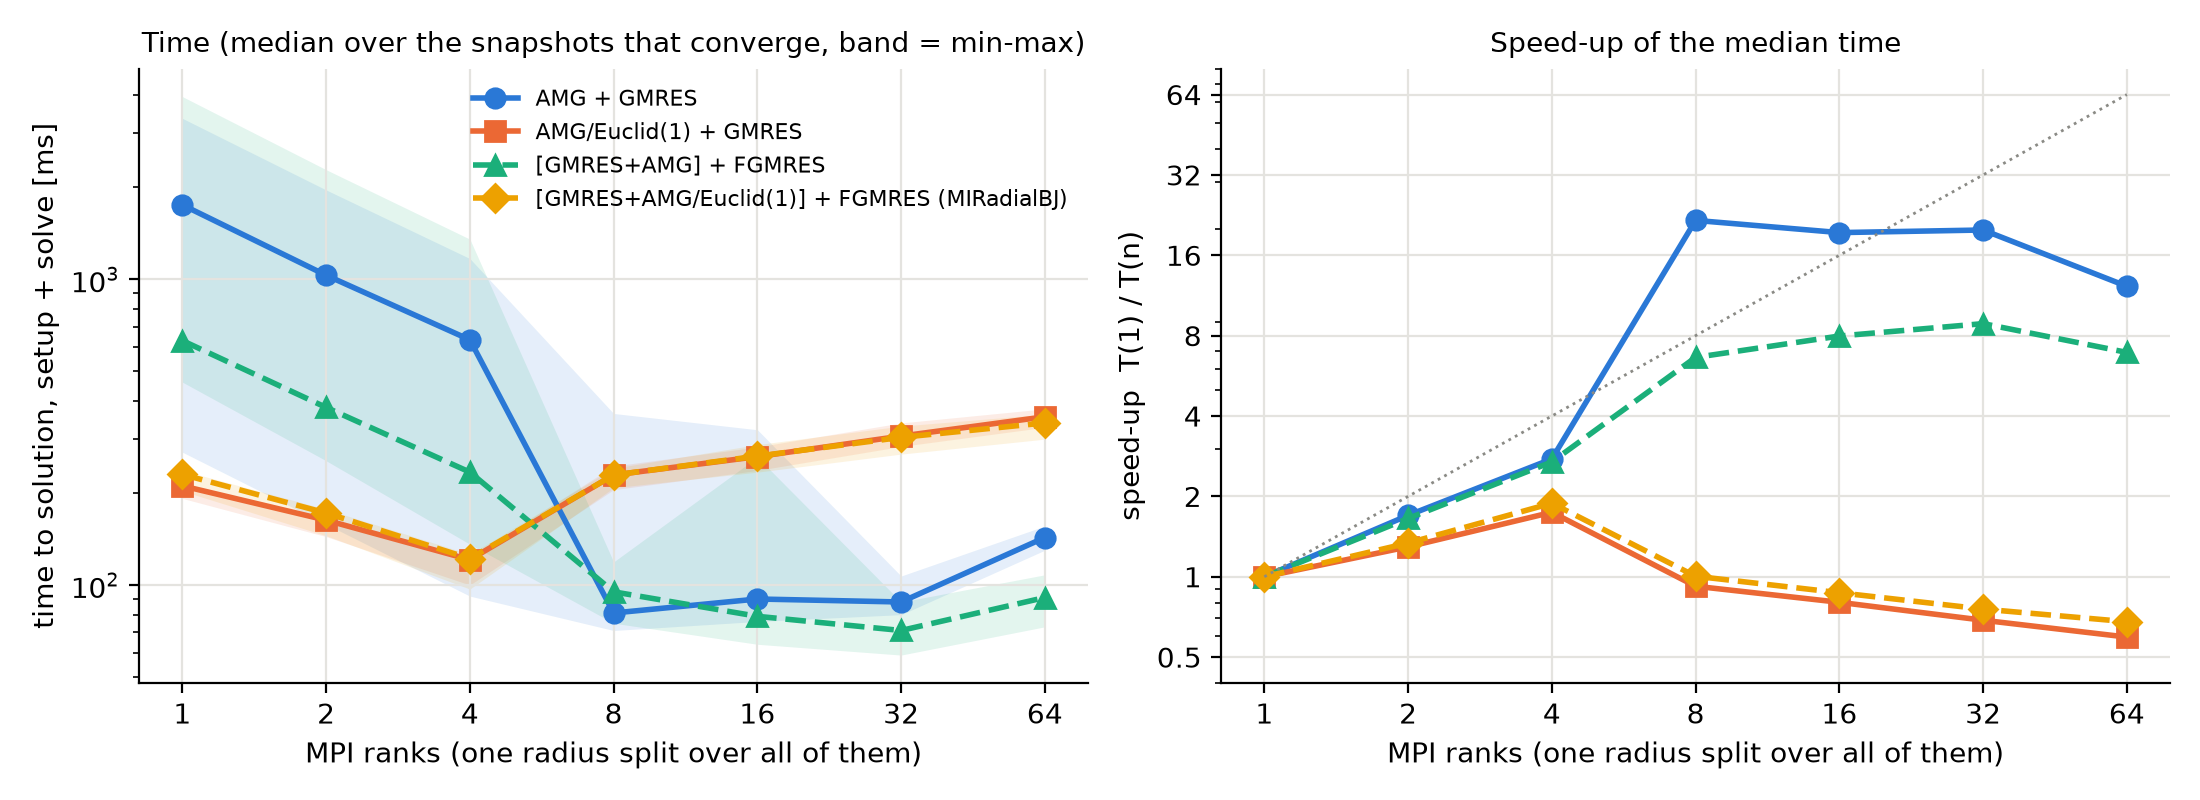
\includegraphics[width=0.95\linewidth]{v5_2919644/scaling_nr1_L2}
    \end{center}
    \vspace{-0.6em}
    \begin{itemize}
        \item time = setup + solve, best of 2 repeats; median over the snapshots that converge;
              speed-up of the median time
        \item AMG + GMRES (default smoother): the jump at 8 ranks is \textbf{not parallel efficiency}:
              its iterations drop from up to 237 (and 2 divergences) on 1--4 ranks to 15--21
    \end{itemize}
\end{frame}

% ---------------------------------------------------------------------
\begin{frame}{Parallel, one radius: results (L2)}
    \footnotesize
    \begin{center}
    \resizebox{\linewidth}{!}{%
    \begin{tabular}{l|rrrrrrr}
        \hline
        median time [ms] (iterations) & 1 & 2 & 4 & 8 & 16 & 32 & 64 \\
        \hline
        AMG + GMRES                 & 1751$^*$ & 1031$^*$ & 634$^*$ & 81 & 90 & 88 & 143 \\
                                    & (20--237) & & & (15--111) & (17--114) & (12--21) & (13--21) \\
        AMG/Euclid(1) + GMRES       & 211 & 163 & \textbf{121} & 229 & 263 & 307 & 355 \\
                                    & (3--4) & (3--4) & (3--4) & (7--9) & (9--12) & (8--14) & (10--12) \\
        {[GMRES+AMG] + FGMRES}      & 630$^*$ & 381$^*$ & 234$^*$ & 95 & 79 & \textbf{71} & 91 \\
        {[GMRES+AMG/Euclid(1)] + FGMRES} & 230 & 172 & \textbf{122} & 229 & 264 & 304 & 339 \\
        \hline
    \end{tabular}}
    \end{center}
    \vspace{-0.4em}
    {\scriptsize FGMRES variants: 2 outer iterations everywhere.
    $^*$ CQ 10\,ms and CQ 29\,ms diverge on 1--4 ranks with the default smoother (not in the median).}
    \begin{itemize}
        \item \textbf{Euclid smoother}: 3--4 iterations, fastest on 1--4 ranks, best speed-up $1.9\times$ at 4 ranks;
              beyond that its parallel ILU setup grows (90\,ms at 4 $\to$ 280\,ms at 64 ranks) and the
              iterations triple: \textbf{slower with more ranks}
        \item \textbf{default smoother}: unreliable on 1--4 ranks, then 71--95\,ms from 8 to 32 ranks,
              slower again at 64
        \item best parallel time $\approx 71$\,ms (32 ranks) vs \textbf{90\,ms for serial ILU(0) + GMRES} on one core
              (previous slides): splitting one radius buys at most $\approx 1.3\times$
        \item $152\,000$ unknowns over 64 ranks is $\approx 2\,400$ rows per rank: communication and
              setup dominate. Parallelism should come from the radius ($N_r \geq$ ranks), not from inside it
        \item to check: AMG + GMRES (default smoother) took 10--11 iterations on the same matrices in the
              serial test, which has no extra \texttt{-scale diag}
    \end{itemize}
\end{frame}

% ---------------------------------------------------------------------
\begin{frame}{Parallel, one radius: speed-up (L4)}
    \footnotesize
    $N_r = 1$, L4 ($2.43$\,M unknowns, 38\,000 rows per rank at 64 ranks), 1 exclusive node,
    8 snapshots (injection end: no reference solution), 2 repeats
    \begin{center}
        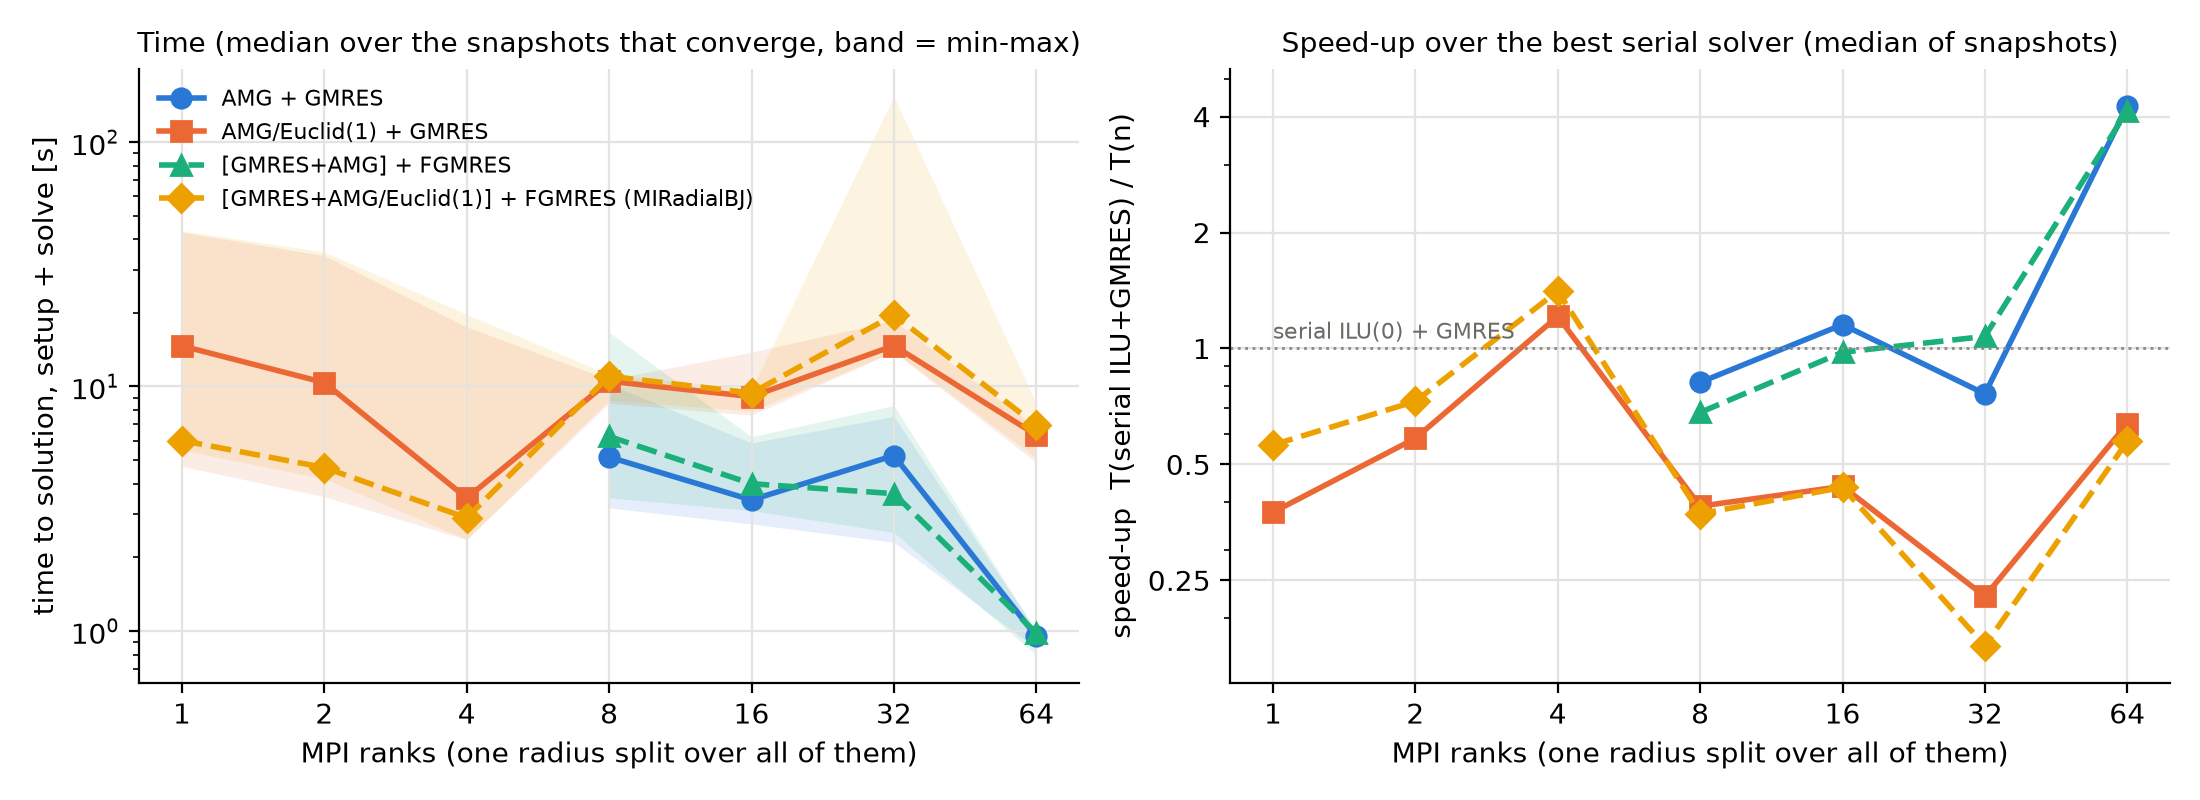
\includegraphics[width=0.95\linewidth]{v5_2919957_L4/scaling_nr1_L4}
    \end{center}
    \vspace{-0.6em}
    \begin{itemize}
        \item speed-up here = per snapshot, time of \textbf{serial ILU(0) + GMRES} (one core, 2.6--7.2\,s) / time on $n$ ranks:
              T(1) does not exist for the default smoother, which fails on 1--4 ranks
        \item a run counts if it converges \textbf{and} its true residual is $\leq 10^{-4}$; no point where more than half of the snapshots fail
    \end{itemize}
\end{frame}

% ---------------------------------------------------------------------
\begin{frame}{Parallel, one radius: results (L4)}
    \footnotesize
    \begin{center}
    \resizebox{\linewidth}{!}{%
    \begin{tabular}{l|rrrrrrr}
        \hline
        median time [s] (iterations) & 1 & 2 & 4 & 8 & 16 & 32 & 64 \\
        \hline
        AMG + GMRES                 & fail 7/8 & fail 7/8 & fail 7/8 & 5.1$^*$ & 3.4 & 5.2 & \textbf{0.95} \\
                                    & & & & (22--133) & (25--121) & (33--252) & (14--20) \\
        AMG/Euclid(1) + GMRES       & 14.7 & 10.4 & 3.5$^*$ & 10.5 & 9.1 & 14.7$^*$ & 6.3$^*$ \\
                                    & (10--206) & (10--206) & (11--206) & (9--15) & (12--109) & (188--292) & (35--61) \\
        {[GMRES+AMG] + FGMRES}      & fail 7/8 & fail 7/8 & fail 7/8 & 6.2$^*$ & 4.0 & 3.6 & \textbf{0.98} \\
        {[GMRES+AMG/Euclid(1)] + FGMRES} & 6.0 & 4.7 & 2.9$^*$ & 11.0 & 9.4 & 19.6$^*$ & 6.9 \\
        \hline
        serial ILU(0) + GMRES (one core) & \multicolumn{7}{l}{4.1 (median), 2.6--6.4} \\
        \hline
    \end{tabular}}
    \end{center}
    \vspace{-0.4em}
    {\scriptsize $^*$ 1--3 of the 8 snapshots fail (not in the median). FGMRES variants: 2 outer iterations.}
    \begin{itemize}
        \item \textbf{default smoother}: fails on 1--4 ranks, converges from 8 on; at \textbf{64 ranks all 8 snapshots
              in 0.8--1.0\,s}: $4\times$ faster than serial ILU(0) + GMRES, $20\times$ faster than serial LU
        \item not monotonic: at 32 ranks AMG + GMRES needs 143--252 iterations (the AMG hierarchy changes with the partition)
        \item \textbf{Euclid smoother}: best at 4 ranks (2.9\,s, $1.4\times$ serial ILU); from 8 ranks its setup jumps
              from 1\,s to 8--10\,s and at 32 ranks 2--3 snapshots fail: \textbf{does not scale}
        \item unlike L2, splitting one radius pays off at L4 (38\,000 rows per rank at 64 ranks), but only with the default smoother
    \end{itemize}
\end{frame}

% ---------------------------------------------------------------------
\begin{frame}{Parallel, one radius: open issues}
    \small
    \begin{itemize}
        \item \textbf{the default smoother fails on 1--4 ranks in the parallel test}
              (L2: 2 of 9 snapshots, L4: 7 of 8), \textbf{but not in the serial test} on the same matrices:
              there AMG + GMRES converges in 7--22 iterations on almost every snapshot
        \begin{itemize}
            \item with one radius both run GMRES + block Jacobi (1 block) + one BoomerAMG V-cycle, right
                  preconditioning; the difference is the extra \texttt{-scale diag} of the parallel test
                  (it solves $D^{-1}A$, which also changes the AMG hierarchy and the stopping test)
            \item until this is understood, the 1--4 rank points of the default smoother are not reliable
        \end{itemize}
        \item \textbf{``converged'' is not enough}: the parallel test stops on the residual of the scaled
              system; at L4, 64 ranks, AMG/Euclid + GMRES reports convergence with true residual $10^{-2}$
              (here counted as a failure; the AMG V-cycle variants often stop at $10^{-6}$--$10^{-5}$)
        \item next: repeat the 1--64 rank scan with \texttt{-scale none} at L2 and L4
    \end{itemize}
\end{frame}
 (update_2026-11-26.tex).

% ---------------------------------------------------------------------
\begin{frame}{Direct vs iterative, one radius: setup}
    \footnotesize
    \begin{itemize}
        \item kinetic system only ($f_\mathrm{hot}$, $f_\mathrm{re}$), \textbf{one radial cell} ($N_r = 1$),
              analytic toroidal geometry, three resolutions
        \begin{itemize}
            \item L1: $N = 38\,000$ unknowns ($f_\mathrm{hot}$ $250 \times 32 = 8\,000$,
                  $f_\mathrm{re}$ $150 \times 200 = 30\,000$), $1.8\times10^{5}$ nonzeros
            \item L2: $N = 152\,000$ ($f_\mathrm{hot}$ $32\,000$ + $f_\mathrm{re}$ $120\,000$),
                  $7.2\times10^{5}$ nonzeros
            \item L4: $N = 2.43$\,M ($f_\mathrm{hot}$ $0.51$\,M + $f_\mathrm{re}$ $1.92$\,M),
                  $1.16\times10^{7}$ nonzeros
            \item no radial coupling: what is left is the momentum-space $(p, \xi)$ operator
        \end{itemize}
        \item all 9 snapshots: injection start / end, CQ at 5, 10, 20, 29, 40, 49\,ms and end
        \begin{itemize}
            \item $\Delta t = 1.8\times10^{-7}$\,s (injection), $1.0\times10^{-7}$\,s (CQ, DREAM substep)
            \item first time step, matrix dumped by \texttt{dreami} (\texttt{-dream\_save\_system})
        \end{itemize}
        \item serial (Pitagora, one core), zero initial guess, restart 100,
              stop at $\|r\|/\|b\| < 10^{-10}$ (true residual)
        \item solvers
        \begin{enumerate}
            \item \textbf{LU}: direct factorization (PETSc's own LU; MUMPS not available in this PETSc build)
            \item \textbf{AMG + GMRES}: one BoomerAMG V-cycle per iteration
            \item \textbf{ILU(0) + GMRES}
            \item \textbf{[GMRES + AMG/Euclid ILU(1)] + FGMRES}: the MIRadialBJ block solver, here with a single block
        \end{enumerate}
    \end{itemize}
\end{frame}

% ---------------------------------------------------------------------
\begin{frame}{Direct vs iterative, one radius: results (serial, L1)}
    \small
    \begin{center}
    \resizebox{\linewidth}{!}{%
    \begin{tabular}{l|r|rr|rr|rr}
        \hline
        & LU & \multicolumn{2}{c|}{AMG + GMRES} & \multicolumn{2}{c|}{ILU(0) + GMRES}
        & \multicolumn{2}{c}{[GMRES+AMG/Eu(1)] + FGMRES} \\
        snapshot & time [ms] & its & time [ms] & its & time [ms] & its (inner) & time [ms] \\
        \hline
        injection start & 123 & 7 & 32 &  9 & \textbf{15} & 2 (6) & 72 \\
        injection end   & 132 & 9 & 39 & 12 & \textbf{18} & 2 (6) & 75 \\
        CQ 5\,ms        & 132 & 8 & 36 & 10 & \textbf{16} & 2 (6) & 76 \\
        CQ 10\,ms       & 174 & 8 & 36 & 10 & \textbf{15} & 2 (6) & 74 \\
        CQ 20\,ms       & 132 & 8 & 36 & 10 & \textbf{15} & 2 (6) & 75 \\
        CQ 29\,ms       & 131 & 7 & 33 &  9 & \textbf{14} & 2 (6) & 76 \\
        CQ 40\,ms       & 131 & 7 & 33 &  9 & \textbf{14} & 2 (6) & 74 \\
        CQ 49\,ms       & 130 & 7 & 33 &  9 & \textbf{14} & 1 (3) & 65 \\
        CQ end          & 129 & 8 & 36 &  8 & \textbf{13} & 2 (4) & 70 \\
        \hline
        relative error  & $\leq 2\times10^{-12}$ & \multicolumn{2}{c|}{$\leq 2\times10^{-10}$}
                        & \multicolumn{2}{c|}{$\leq 2\times10^{-11}$} & \multicolumn{2}{c}{$\leq 4\times10^{-11}$} \\
        \hline
    \end{tabular}}
    \end{center}
    \vspace{0.3em}
    \begin{itemize}
        \item time = setup + solve; error = $\|x - x_\mathrm{ref}\| / \|x_\mathrm{ref}\|$,
              $x_\mathrm{ref}$ = \texttt{dreami}'s solution
        \item every solver converges on every snapshot
        \item LU: factorization 122--173\,ms, triangular solves 1\,ms
        \item block-Jacobi variants with one block give the same iterations and residuals
              as the global ones (consistency check)
    \end{itemize}
\end{frame}

% ---------------------------------------------------------------------
\begin{frame}{Direct vs iterative, one radius: results (serial, L2)}
    \small
    \begin{center}
    \resizebox{\linewidth}{!}{%
    \begin{tabular}{l|r|rr|rr|rr}
        \hline
        & LU & \multicolumn{2}{c|}{AMG + GMRES} & \multicolumn{2}{c|}{ILU(0) + GMRES}
        & \multicolumn{2}{c}{[GMRES+AMG/Eu(1)] + FGMRES} \\
        snapshot & time [ms] & its & time [ms] & its & time [ms] & its (inner) & time [ms] \\
        \hline
        injection start & 638 & 10 & 167 & 15 & \textbf{92}  & 2 (18) & 380 \\
        injection end   & 720 & 11 & 186 & 19 & \textbf{116} & 2 (6)  & 281 \\
        CQ 5\,ms        & 709 & 11 & 182 & 15 & \textbf{91}  & 2 (6)  & 281 \\
        CQ 10\,ms       & 709 & 11 & 181 & 15 & \textbf{90}  & 2 (6)  & 280 \\
        CQ 20\,ms       & 703 & 11 & 183 & 14 & \textbf{86}  & 2 (6)  & 281 \\
        CQ 29\,ms       & 706 & 11 & 183 & 14 & \textbf{86}  & 2 (6)  & 274 \\
        CQ 40\,ms       & 701 & 11 & 186 & 14 & \textbf{85}  & 2 (6)  & 287 \\
        CQ 49\,ms       & 690 & \textbf{58} & \textbf{928} & 13 & \textbf{82} & 2 (6) & 274 \\
        CQ end          & 667 & 10 & 166 & 11 & \textbf{69}  & 2 (6)  & 258 \\
        \hline
        relative error  & $\leq 3\times10^{-12}$ & \multicolumn{2}{c|}{$\leq 5\times10^{-9}$}
                        & \multicolumn{2}{c|}{$\leq 5\times10^{-10}$} & \multicolumn{2}{c}{$\leq 3\times10^{-12}$} \\
        \hline
    \end{tabular}}
    \end{center}
    \vspace{0.3em}
    \begin{itemize}
        \item every solver converges on every snapshot
        \item LU: factorization 0.63--0.71\,s, triangular solves 6\,ms
        \item AMG + GMRES at CQ 49\,ms: 58 iterations, and its true residual $9\times10^{-10}$
              stays above the $10^{-10}$ target (error $5\times10^{-9}$)
    \end{itemize}
\end{frame}

% ---------------------------------------------------------------------
\begin{frame}{Direct vs iterative, one radius: results (serial, L4)}
    \small
    \begin{center}
    \resizebox{\linewidth}{!}{%
    \begin{tabular}{l|r|rr|rr|rr}
        \hline
        & LU & \multicolumn{2}{c|}{AMG + GMRES} & \multicolumn{2}{c|}{ILU(0) + GMRES}
        & \multicolumn{2}{c}{[GMRES+AMG/Eu(1)] + FGMRES} \\
        snapshot & time [s] & its & time [s] & its & time [s] & its (inner) & time [s] \\
        \hline
        injection start & 17.5 & \textbf{104} & \textbf{31.2} & 56 & \textbf{6.4} & 2 (\textbf{260}) & \textbf{60.1} \\
        injection end   & 22.0 & 14  & \textbf{4.5}  & 61 & 7.2  & 2 (7) & 5.4 \\
        CQ 5\,ms        & 21.1 & 13  & \textbf{4.0}  & 40 & 4.4  & 2 (6) & 5.0 \\
        CQ 10\,ms       & 21.0 & 22  & 6.4  & 40 & \textbf{4.2}  & 2 (6) & 5.0 \\
        CQ 20\,ms       & 20.9 & 13  & \textbf{4.0}  & 39 & 4.2  & 2 (6) & 5.0 \\
        CQ 29\,ms       & 21.0 & \textbf{107} & \textbf{33.6} & 38 & \textbf{4.1} & 2 (6) & 4.9 \\
        CQ 40\,ms       & 20.8 & 13  & 4.0  & 37 & \textbf{3.9}  & 2 (6) & 4.8 \\
        CQ 49\,ms       & 20.3 & 13  & 4.0  & 31 & \textbf{3.3}  & 2 (6) & 4.8 \\
        CQ end          & 18.3 & 13  & 3.8  & 26 & \textbf{2.6}  & 2 (6) & 4.5 \\
        \hline
        relative error  & $\leq 7\times10^{-11}$ & \multicolumn{2}{c|}{$\leq 5\times10^{-10}$}
                        & \multicolumn{2}{c|}{$\leq 6\times10^{-10}$} & \multicolumn{2}{c}{$\leq 6\times10^{-11}$} \\
        \hline
    \end{tabular}}
    \end{center}
    \vspace{0.3em}
    \begin{itemize}
        \item every solver converges on every snapshot (injection end: no reference solution, no error)
        \item LU: factorization 17--22\,s, triangular solves 0.13\,s
        \item AMG + GMRES and the MIRadialBJ block solver have outliers ($8\times$ / $12\times$ slower);
              ILU(0) + GMRES has none, but its iterations grow with the resolution (26--61)
        \item true residual $\approx 10^{-8}$ for every solver, LU included: the floor of these systems at L4
    \end{itemize}
\end{frame}

% ---------------------------------------------------------------------
\begin{frame}{Direct vs iterative, one radius: conclusions}
    \footnotesize
    \begin{center}
    \begin{tabular}{l|rr|r}
        \hline
        total time, range over the 9 snapshots & L1 [ms] & L2 [ms] & L4 [s] \\
        \hline
        LU                                  & 123--174 & 638--720 & 17.5--22.0 \\
        AMG + GMRES                         & 32--39   & 166--186 (928) & 3.8--6.4 (31, 34) \\
        ILU(0) + GMRES                      & \textbf{13--18} & \textbf{69--116} & \textbf{2.6--7.2} \\
        {[GMRES+AMG/Eu(1)] + FGMRES}        & 65--76   & 258--380 & 4.5--5.4 (60) \\
        \hline
        unknowns                            & 38\,k & 152\,k & 2.43\,M \\
        \hline
    \end{tabular}
    \end{center}
    \vspace{0.2em}
    \begin{itemize}
        \item \textbf{ILU(0) + GMRES is the fastest and the only one without outliers}: $8$--$9\times$ faster
              than LU at L1--L2, $\approx 5\times$ at L4; at L4 AMG + GMRES is as fast on most snapshots;
              ILU iterations grow with the resolution: 8--12 (L1), 11--19 (L2), 26--61 (L4)
        \item \textbf{LU is the slowest}: almost all the time is the factorization; it would pay off
              only if reused for $\gtrsim 10$ solves, but the matrix changes at every time step
        \item \textbf{AMG + GMRES is not robust}: 7--22 iterations, except 58 (L2, CQ 49\,ms)
              and 104--107 (L4, injection start, CQ 29\,ms)
        \item the MIRadialBJ block solver: 2 outer iterations on every snapshot and level, but its
              AMG + Euclid setup dominates (50\,ms L1, 200\,ms L2, 3.4\,s L4); L4 injection start: 260 inner its
    \end{itemize}
    \vspace{0.2em}
    \textbf{Caveat}: easy systems ($\Delta t \approx 10^{-7}$\,s, no radial coupling); with $N_r = 11$ at L2 (v4)
    ILU(0) needed 150--238 iterations. Next: full source step ($\Delta t \approx 10^{-4}$\,s), LU with MUMPS
\end{frame}

% =====================================================================
% Parallel: one radius split over the MPI ranks
% =====================================================================
\begin{frame}{Parallel, one radius: speed-up (L2)}
    \footnotesize
    $N_r = 1$, L2 ($152\,000$ unknowns): the single radius block is split over all $n$ ranks
    (1 exclusive node, $n = 1 \dots 64$), solved by a parallel BoomerAMG; 9 snapshots, 2 repeats
    \begin{center}
        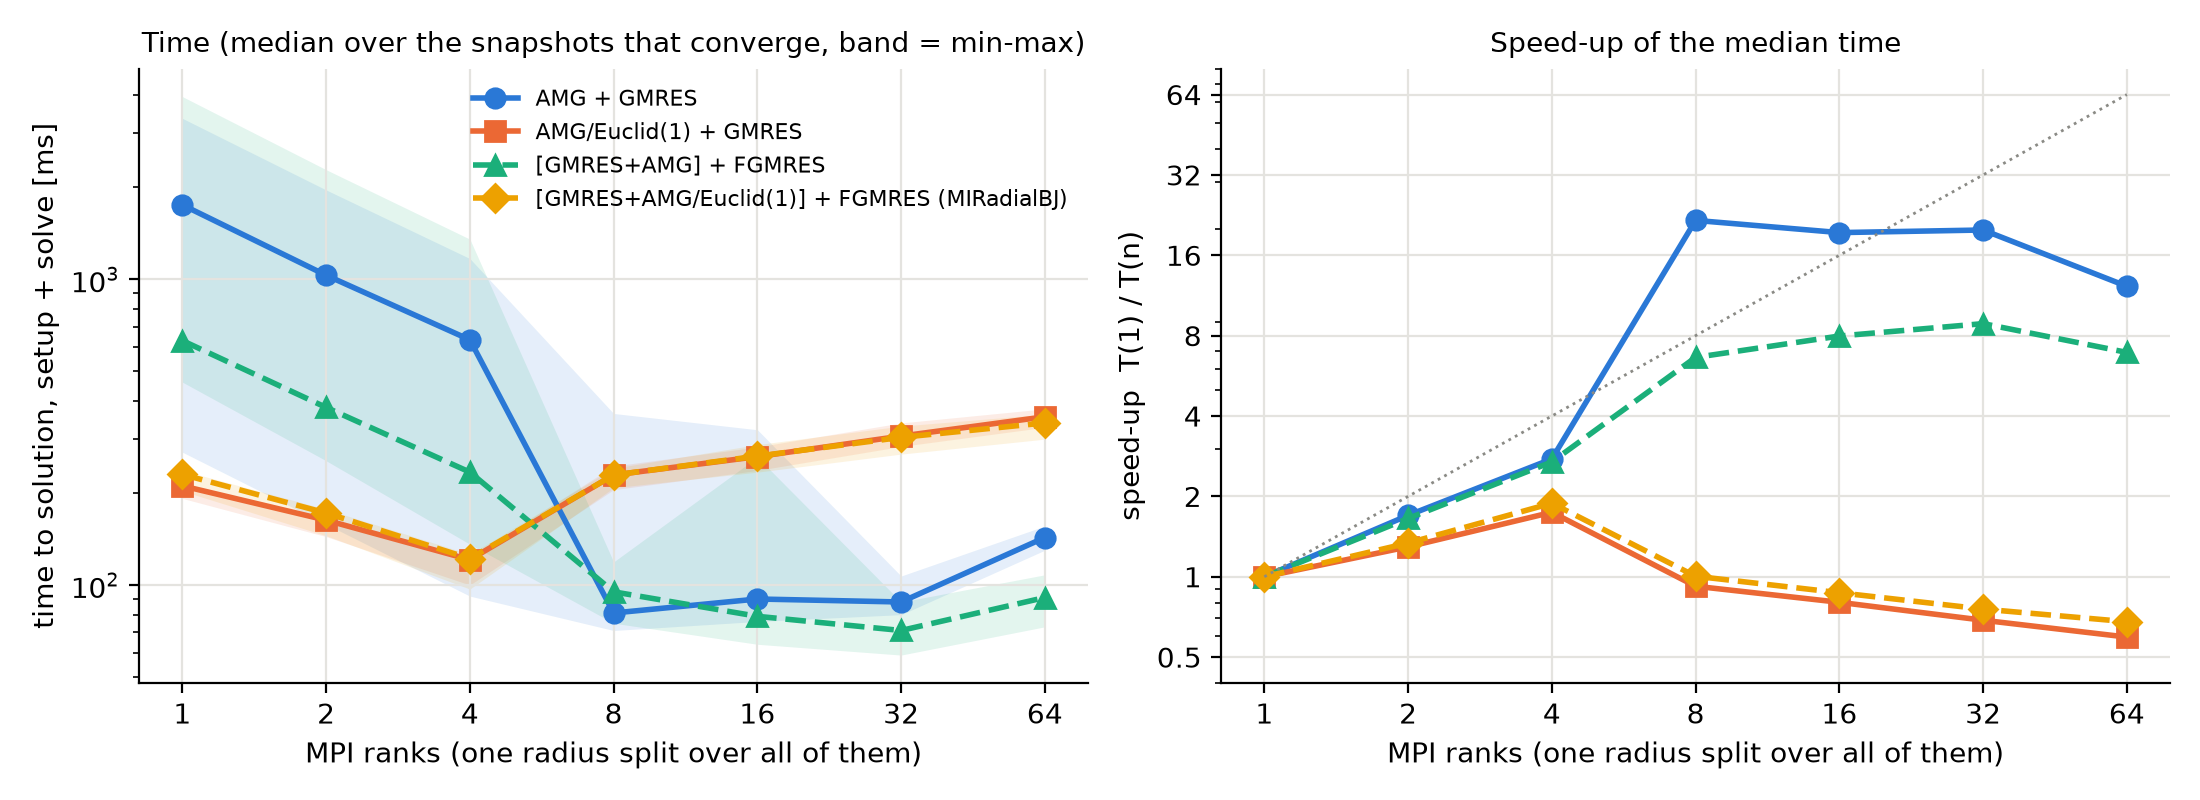
\includegraphics[width=0.95\linewidth]{v5_2919644/scaling_nr1_L2}
    \end{center}
    \vspace{-0.6em}
    \begin{itemize}
        \item time = setup + solve, best of 2 repeats; median over the snapshots that converge;
              speed-up of the median time
        \item AMG + GMRES (default smoother): the jump at 8 ranks is \textbf{not parallel efficiency}:
              its iterations drop from up to 237 (and 2 divergences) on 1--4 ranks to 15--21
    \end{itemize}
\end{frame}

% ---------------------------------------------------------------------
\begin{frame}{Parallel, one radius: results (L2)}
    \footnotesize
    \begin{center}
    \resizebox{\linewidth}{!}{%
    \begin{tabular}{l|rrrrrrr}
        \hline
        median time [ms] (iterations) & 1 & 2 & 4 & 8 & 16 & 32 & 64 \\
        \hline
        AMG + GMRES                 & 1751$^*$ & 1031$^*$ & 634$^*$ & 81 & 90 & 88 & 143 \\
                                    & (20--237) & & & (15--111) & (17--114) & (12--21) & (13--21) \\
        AMG/Euclid(1) + GMRES       & 211 & 163 & \textbf{121} & 229 & 263 & 307 & 355 \\
                                    & (3--4) & (3--4) & (3--4) & (7--9) & (9--12) & (8--14) & (10--12) \\
        {[GMRES+AMG] + FGMRES}      & 630$^*$ & 381$^*$ & 234$^*$ & 95 & 79 & \textbf{71} & 91 \\
        {[GMRES+AMG/Euclid(1)] + FGMRES} & 230 & 172 & \textbf{122} & 229 & 264 & 304 & 339 \\
        \hline
    \end{tabular}}
    \end{center}
    \vspace{-0.4em}
    {\scriptsize FGMRES variants: 2 outer iterations everywhere.
    $^*$ CQ 10\,ms and CQ 29\,ms diverge on 1--4 ranks with the default smoother (not in the median).}
    \begin{itemize}
        \item \textbf{Euclid smoother}: 3--4 iterations, fastest on 1--4 ranks, best speed-up $1.9\times$ at 4 ranks;
              beyond that its parallel ILU setup grows (90\,ms at 4 $\to$ 280\,ms at 64 ranks) and the
              iterations triple: \textbf{slower with more ranks}
        \item \textbf{default smoother}: unreliable on 1--4 ranks, then 71--95\,ms from 8 to 32 ranks,
              slower again at 64
        \item best parallel time $\approx 71$\,ms (32 ranks) vs \textbf{90\,ms for serial ILU(0) + GMRES} on one core
              (previous slides): splitting one radius buys at most $\approx 1.3\times$
        \item $152\,000$ unknowns over 64 ranks is $\approx 2\,400$ rows per rank: communication and
              setup dominate. Parallelism should come from the radius ($N_r \geq$ ranks), not from inside it
        \item to check: AMG + GMRES (default smoother) took 10--11 iterations on the same matrices in the
              serial test, which has no extra \texttt{-scale diag}
    \end{itemize}
\end{frame}

% ---------------------------------------------------------------------
\begin{frame}{Parallel, one radius: speed-up (L4)}
    \footnotesize
    $N_r = 1$, L4 ($2.43$\,M unknowns, 38\,000 rows per rank at 64 ranks), 1 exclusive node,
    8 snapshots (injection end: no reference solution), 2 repeats
    \begin{center}
        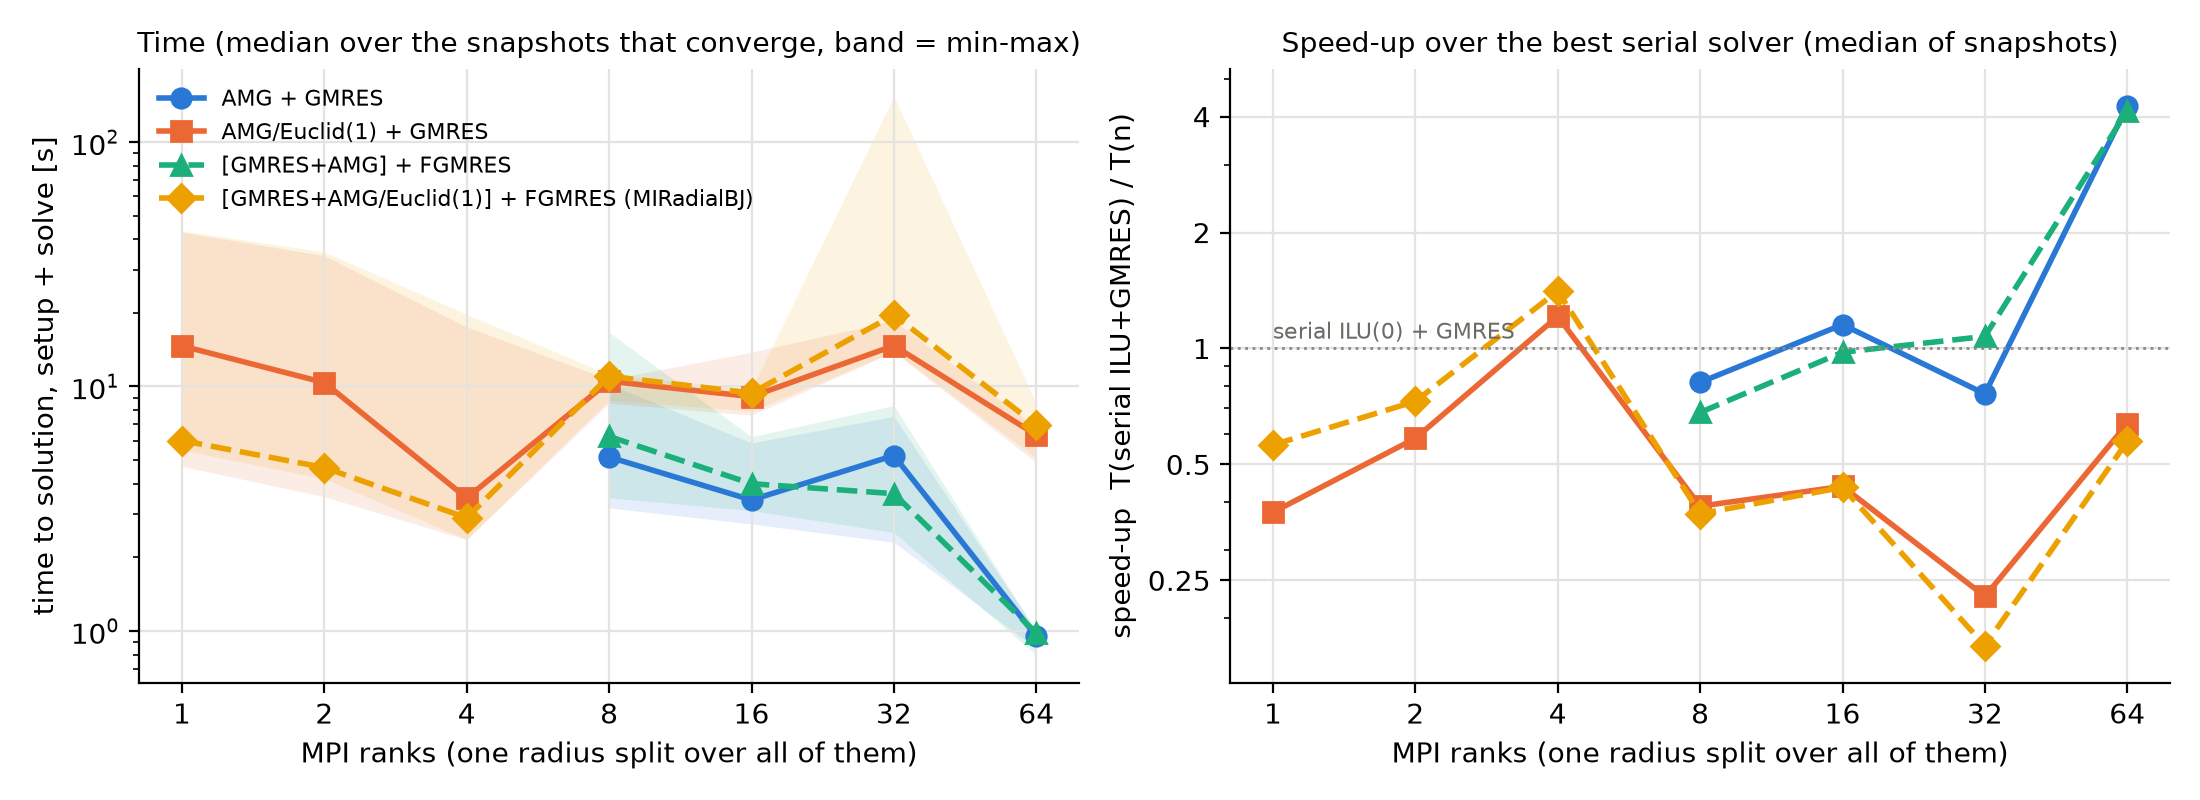
\includegraphics[width=0.95\linewidth]{v5_2919957_L4/scaling_nr1_L4}
    \end{center}
    \vspace{-0.6em}
    \begin{itemize}
        \item speed-up here = per snapshot, time of \textbf{serial ILU(0) + GMRES} (one core, 2.6--7.2\,s) / time on $n$ ranks:
              T(1) does not exist for the default smoother, which fails on 1--4 ranks
        \item a run counts if it converges \textbf{and} its true residual is $\leq 10^{-4}$; no point where more than half of the snapshots fail
    \end{itemize}
\end{frame}

% ---------------------------------------------------------------------
\begin{frame}{Parallel, one radius: results (L4)}
    \footnotesize
    \begin{center}
    \resizebox{\linewidth}{!}{%
    \begin{tabular}{l|rrrrrrr}
        \hline
        median time [s] (iterations) & 1 & 2 & 4 & 8 & 16 & 32 & 64 \\
        \hline
        AMG + GMRES                 & fail 7/8 & fail 7/8 & fail 7/8 & 5.1$^*$ & 3.4 & 5.2 & \textbf{0.95} \\
                                    & & & & (22--133) & (25--121) & (33--252) & (14--20) \\
        AMG/Euclid(1) + GMRES       & 14.7 & 10.4 & 3.5$^*$ & 10.5 & 9.1 & 14.7$^*$ & 6.3$^*$ \\
                                    & (10--206) & (10--206) & (11--206) & (9--15) & (12--109) & (188--292) & (35--61) \\
        {[GMRES+AMG] + FGMRES}      & fail 7/8 & fail 7/8 & fail 7/8 & 6.2$^*$ & 4.0 & 3.6 & \textbf{0.98} \\
        {[GMRES+AMG/Euclid(1)] + FGMRES} & 6.0 & 4.7 & 2.9$^*$ & 11.0 & 9.4 & 19.6$^*$ & 6.9 \\
        \hline
        serial ILU(0) + GMRES (one core) & \multicolumn{7}{l}{4.1 (median), 2.6--6.4} \\
        \hline
    \end{tabular}}
    \end{center}
    \vspace{-0.4em}
    {\scriptsize $^*$ 1--3 of the 8 snapshots fail (not in the median). FGMRES variants: 2 outer iterations.}
    \begin{itemize}
        \item \textbf{default smoother}: fails on 1--4 ranks, converges from 8 on; at \textbf{64 ranks all 8 snapshots
              in 0.8--1.0\,s}: $4\times$ faster than serial ILU(0) + GMRES, $20\times$ faster than serial LU
        \item not monotonic: at 32 ranks AMG + GMRES needs 143--252 iterations (the AMG hierarchy changes with the partition)
        \item \textbf{Euclid smoother}: best at 4 ranks (2.9\,s, $1.4\times$ serial ILU); from 8 ranks its setup jumps
              from 1\,s to 8--10\,s and at 32 ranks 2--3 snapshots fail: \textbf{does not scale}
        \item unlike L2, splitting one radius pays off at L4 (38\,000 rows per rank at 64 ranks), but only with the default smoother
    \end{itemize}
\end{frame}

% ---------------------------------------------------------------------
\begin{frame}{Parallel, one radius: open issues}
    \small
    \begin{itemize}
        \item \textbf{the default smoother fails on 1--4 ranks in the parallel test}
              (L2: 2 of 9 snapshots, L4: 7 of 8), \textbf{but not in the serial test} on the same matrices:
              there AMG + GMRES converges in 7--22 iterations on almost every snapshot
        \begin{itemize}
            \item with one radius both run GMRES + block Jacobi (1 block) + one BoomerAMG V-cycle, right
                  preconditioning; the difference is the extra \texttt{-scale diag} of the parallel test
                  (it solves $D^{-1}A$, which also changes the AMG hierarchy and the stopping test)
            \item until this is understood, the 1--4 rank points of the default smoother are not reliable
        \end{itemize}
        \item \textbf{``converged'' is not enough}: the parallel test stops on the residual of the scaled
              system; at L4, 64 ranks, AMG/Euclid + GMRES reports convergence with true residual $10^{-2}$
              (here counted as a failure; the AMG V-cycle variants often stop at $10^{-6}$--$10^{-5}$)
        \item next: repeat the 1--64 rank scan with \texttt{-scale none} at L2 and L4
    \end{itemize}
\end{frame}
